\documentclass[12pt]{article}
%\usepackage[utf8]{inputenc}
%\documentclass[UTF8]{ctexart}
%\usepackage[UTF8, heading = false, scheme = plain]{ctex}
\usepackage{geometry}
%geometry{a4paper,scale=0.9}
\geometry{a4paper,left=1cm,right=1cm,top=1cm,bottom=2cm}
\usepackage{amsfonts}
\usepackage{color}
\usepackage{url}
%\usepackage{biblatex}
\usepackage{amsmath}
\usepackage{amssymb}
\usepackage{latexsym}
\usepackage{cite}
%\addbibresource{ref.bib}
%\bibliography{ref.bib}
\usepackage{caption}
\usepackage{graphicx, subfig}
\usepackage{float}
%\usepackage[fontset=ubuntu]{ctex}
%\usepackage{fontspec}
\usepackage{xeCJK}
%\usepackage[colorlinks,
%anchorcolor=black,
%citecolor=black]{hyperref}
%\setmainfont{SimSun}
\usepackage[section]{placeins}
\usepackage{enumitem}
\usepackage{framed}
\usepackage[framemethod=TikZ]{mdframed}
\usepackage{indentfirst}
\usepackage{setspace}%使用间距宏包
\linespread{1.5}
%\title{预备知识}
%\author{leolinuxer }
%\date{June 2020}

\title{线性代数基础要点}
\author{leolinuxer}
%\date{June 2020}

\begin{document}
\maketitle
\tableofcontents

\section{线性代数解决什么问题\cite{Why_Learn_Linear_Algebra}}
线性代数研究的是\textbf{如何解决线性问题};如何\textbf{把复杂问题线性化}是别的学科的内容,比如《微积分》、《信号与系统》等。

线性代数讨论的线性问题包括:
\begin{itemize}
\setlength{\itemsep}{0pt}
\setlength{\parsep}{0pt}
\setlength{\parskip}{0pt}
    \item 向量、向量空间:
    \item \textbf{关于向量、向量空间的函数},也称为矩阵函数;矩阵可以对向量进行变换
    \item 对矩阵函数进行坐标变换
\end{itemize}

\subsection{线性代数的几个基础概念和他们之间的关系}
\begin{itemize}
\setlength{\itemsep}{0pt}
\setlength{\parsep}{0pt}
\setlength{\parskip}{0pt}
    \item \textbf{「基」}
    \item \textbf{向量}:描述线性的“东西”(直线、平面、立方体);
    \item \textbf{矩阵}可以对向量进行变换;变换的形式包括:
    \begin{itemize}
    \setlength{\itemsep}{0pt}
    \setlength{\parsep}{0pt}
    \setlength{\parskip}{0pt}
        \item \textbf{线性变换}:旋转、推移、伸缩;投影之类的\textbf{升降维}的操作;恒等变换(单位变换)、求微商(线性空间$P[x]$内)、求定积分等
        \item \textbf{仿射变换}:线性变换+平移
    \end{itemize}
    \item \textbf{行列式}:代表矩阵变换前后的面积(体积)之比
    \item \textbf{「秩」}
    \item \textbf{相似矩阵}
    \item \textbf{二次型}
    \item \textbf{特征值和特征向量}
    \item \textbf{「迹」}
    \item \textbf{奇异值}
\end{itemize}

\section{矩阵\cite{How_To_Understand_Matrix_Multiplication}}
\textcolor{red}{正确的观点是把矩阵看作函数,这样很多疑惑就可以迎刃而解。}

\subsection{矩阵是一个函数}
我们熟悉的直线函数 $ax = y$,把点 $(x,0)$ 映射到 点$(0,ax)$。

我们通过矩阵:$A\vec{x} = \vec{y}$ 也可以完成这个映射,令:
$$
A=
\begin{pmatrix}
0&1\\a&0
\end{pmatrix}
$$

也可以完成:
$$
A\vec{x}=
\begin{pmatrix}
0&1\\a&0
\end{pmatrix}
\begin{pmatrix}
x\\0
\end{pmatrix}
=
\begin{pmatrix}
0\\ax
\end{pmatrix}
$$

对于:$ax=y,x\in\mathbb{R},y\in\mathbb{R}$ 只能完成实数到实数的映射:
$x\to y\implies \mathbb{R}\to\mathbb{R}$

但是对于:$A\vec{x}=\vec{y},\vec{x}\in\mathbb{R}^n,\vec{y}\in\mathbb{R}^m$可以完成更广泛的映射:
$\vec{x}\to \vec{y}\implies \mathbb{R}^n\to\mathbb{R}^m$

\textbf{为了完成这一点,矩阵$A$就不再是系数$a$了,而是一个函数(或者说是映射)。}

写成这样,矩阵乘法看起来更像是函数:$A(\vec{x})=\vec{y}$

\begin{framed}  
%\verb|\documentstyle[ifthen,12pt,titlepage]{article}|
\small{
从线性方程组的角度来看,也很容易得出矩阵是一个函数的结论来。给定线性方程组
$$
\begin{cases}
y_1 = x_1 + 2x_2 \\
y_2 = 2x_1 + x_2
\end{cases}
$$

按照矩阵形式,可以改写为:
$$
\begin{bmatrix}
y_1 \\ y_2
\end{bmatrix} = 
\begin{bmatrix}
1 & 2 \\ 2 & 1
\end{bmatrix}
\begin{bmatrix}
x_1 \\ x_2
\end{bmatrix}
$$

所以,矩阵$[1,2;2,1]$ 就是一个线性变换的函数。
}
\end{framed}

\subsection{矩阵也被称为线性映射}
假设$\vec{x}$所在平面为$V$,而$\vec{y}$所在平面为$W$,$\vec{x}$通过矩阵$A$映射到了$\vec{y}$,可以如下表示:
\begin{figure}[H]
\centering
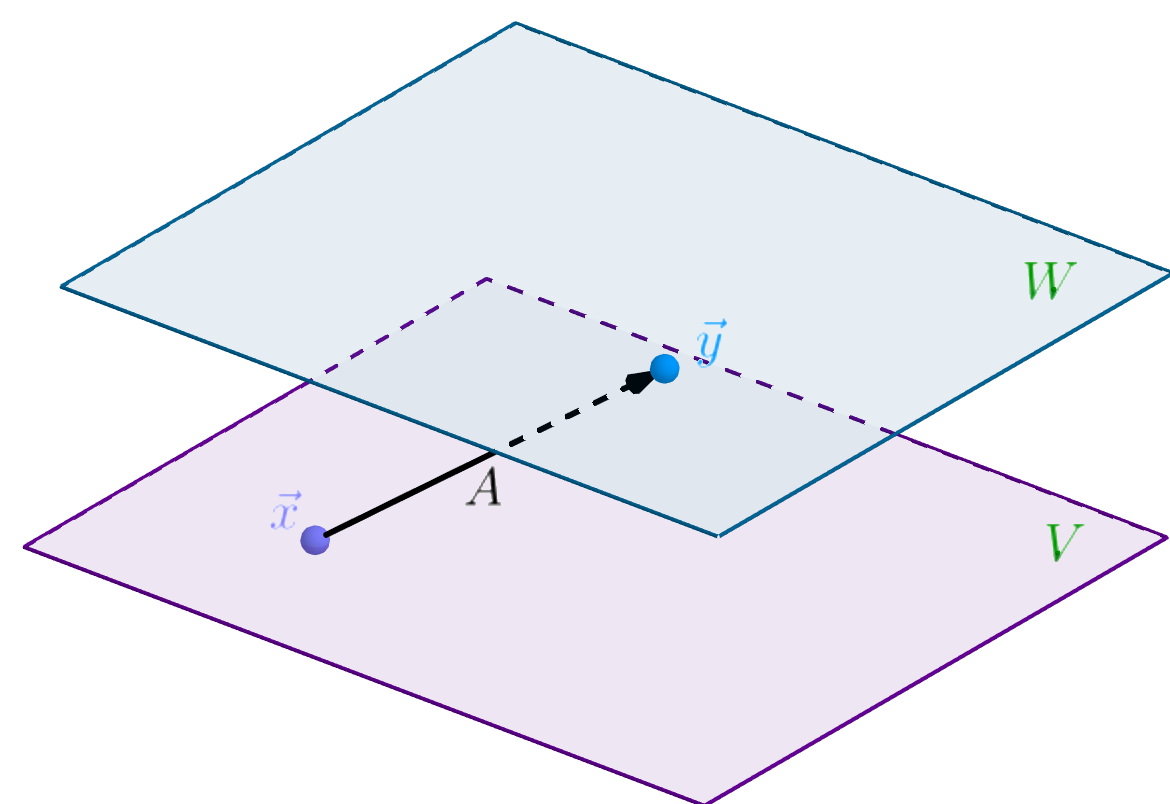
\includegraphics[width=.3\textwidth]{fig/UnderstandMatrixMultiplication_1.png} 
\end{figure}

$A$这个映射的特殊之处是,$V$上的直线通过$A$映射到$W$上也是直线:
\begin{figure}[H]
\centering
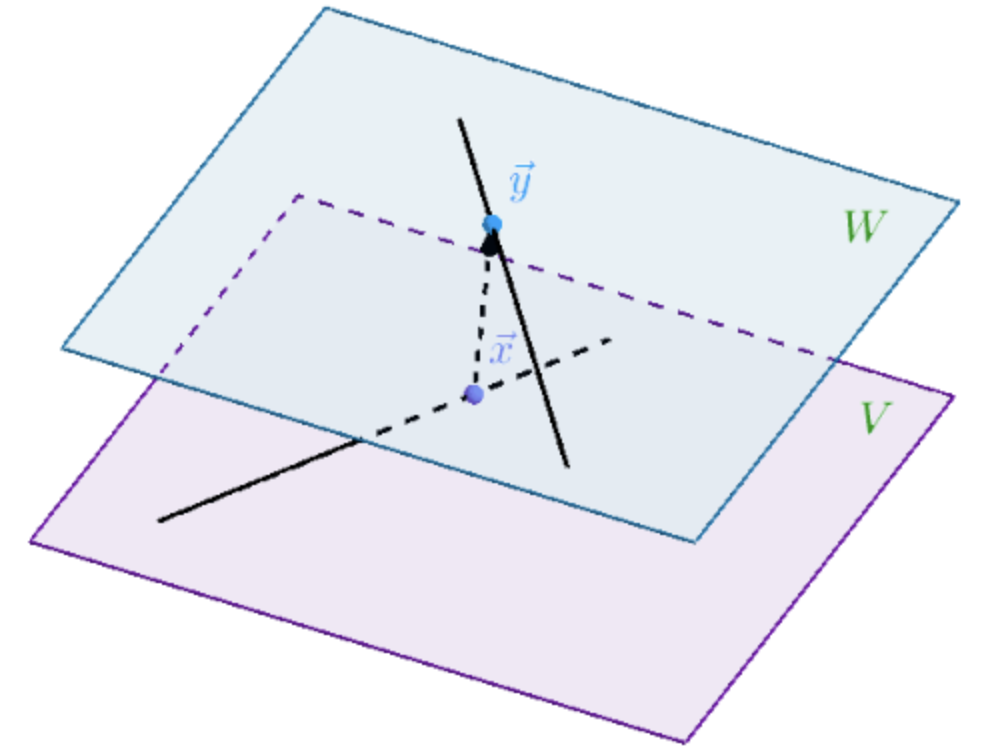
\includegraphics[width=.3\textwidth]{fig/UnderstandMatrixMultiplication_2.png}
\end{figure}

所以矩阵也被称为线性映射。

\subsection{矩阵函数的工作方式}
我们来看看矩阵$A$是如何工作的。为了方便后面的讲解,把之前表示线性映射的3D图变为2D图:
\begin{figure}[H]
\centering
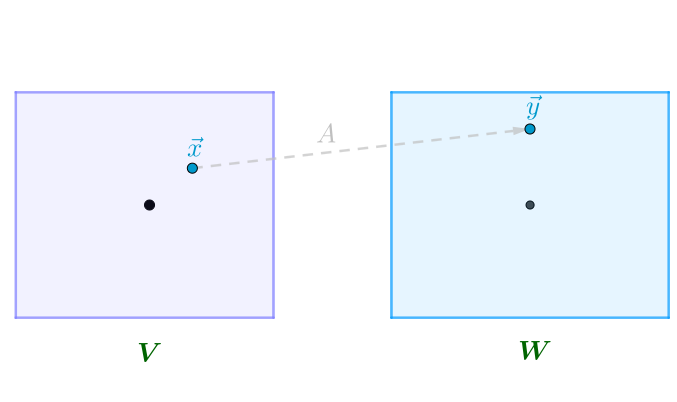
\includegraphics[width=.5\textwidth]{fig/UnderstandMatrixMultiplication_3.png}
\end{figure}

为了画图方便,$\vec{x}$所在平面为$V$、$\vec{y}$所在平面为$W$,都是二维平面,即$\mathbb{R}^2$。

\subsubsection{坐标}
研究线性映射,最重要的是搞清楚当前处在哪个基下。我们先来看看:
$\vec{x}=\begin{pmatrix}x_1\\x_2\end{pmatrix},\vec{y}=\begin{pmatrix}y_1\\y_2\end{pmatrix}$的基。

$\vec{x},\vec{y}$的基默认为各自向量空间下的自然基,其自然基为(即$\mathbb{R}^2$下的自然基):
$$\vec{i}=\begin{pmatrix}1\\0\end{pmatrix}\qquad\vec{j}=\begin{pmatrix}0\\1\end{pmatrix}$$

所以:
$$\vec{x}=x_1\vec{i}+x_2\vec{j}\qquad\vec{y}=y_1\vec{i}+y_2\vec{j}$$
\begin{figure}[H]
\centering
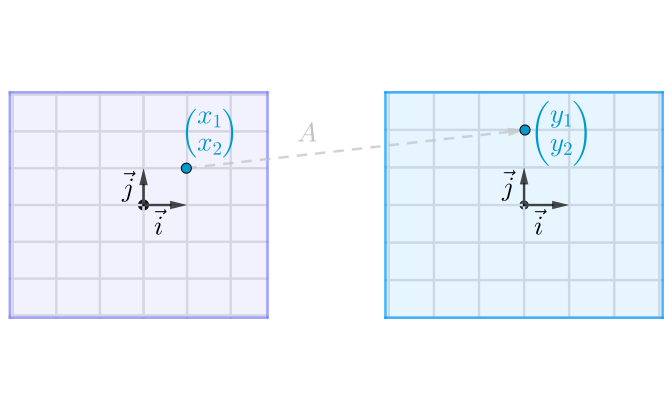
\includegraphics[width=.5\textwidth]{fig/UnderstandMatrixMultiplication_4.png}
\end{figure}

\subsubsection{映射法则的工作原理}
为了说清楚映射法则$A$是怎么工作的,我们把$A$也用一个空间表示,$V$会通过$A$映射到$W$:
\begin{figure}[H]
\centering
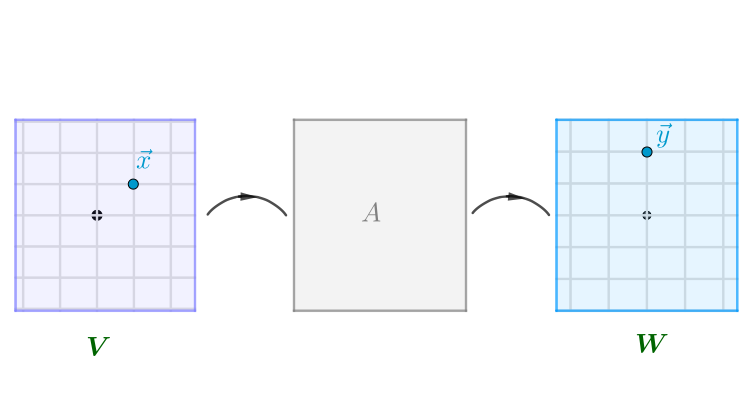
\includegraphics[width=.5\textwidth]{fig/UnderstandMatrixMultiplication_5.png}
\end{figure}

若:$A=\begin{pmatrix}\vec{c_1},&\vec{c_2}\end{pmatrix}$其中$\vec{c_1},\vec{c_2}$为$A$的列向量。
根据矩阵乘法的规则有:
$A\vec{x}=x_1\vec{c_1}+x_2\vec{c_2}$
则\textbf{$A\vec{x}$相当于在$A$空间中,以$\vec{c_1},\vec{c_2}$为基,坐标为$\begin{pmatrix}x_1\\x_2\end{pmatrix}$的向量}:
\begin{figure}[H]
\centering
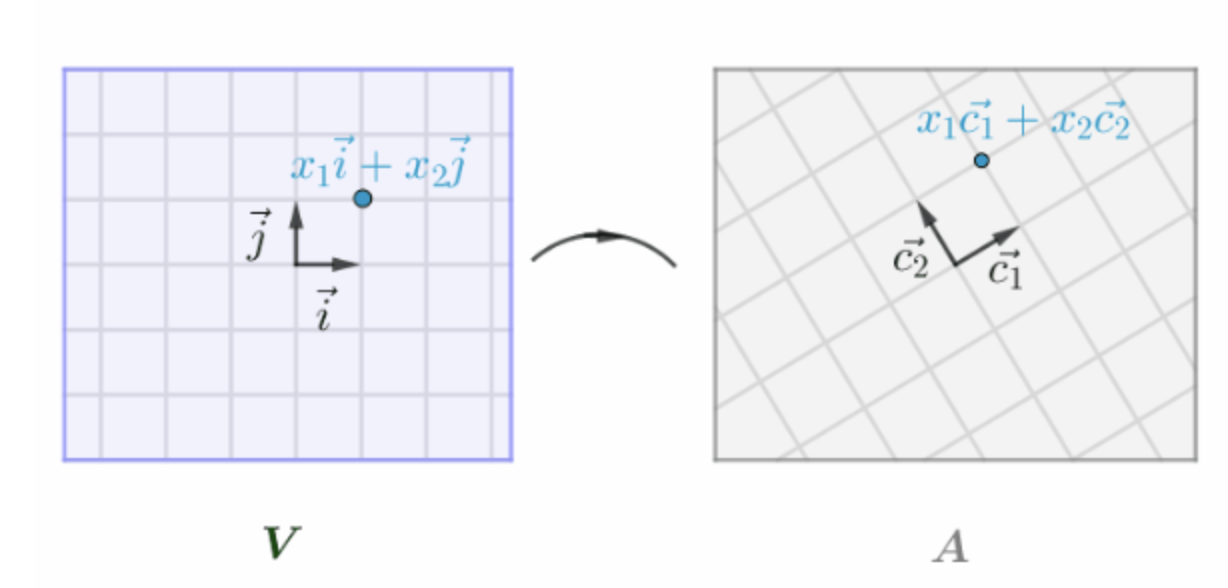
\includegraphics[width=.8\textwidth]{fig/UnderstandMatrixMultiplication_6.png}
\end{figure}

\begin{framed}  
%\verb|\documentstyle[ifthen,12pt,titlepage]{article}|
\small{
举例说明 $A\vec{x}=x_1\vec{c_1}+x_2\vec{c_2}$:
$$
A = 
\begin{pmatrix}
\vec{c_1},&\vec{c_2}
\end{pmatrix} = 
\begin{pmatrix}
c_{11}&c_{12} \\
c_{21}&c_{22}
\end{pmatrix} 
$$
$$
A\vec{x} = 
\begin{pmatrix}
c_{11}&c_{12} \\
c_{21}&c_{22}
\end{pmatrix} 
\begin{pmatrix}
x_1 \\
x_2
\end{pmatrix} = 
\begin{pmatrix}
c_{11}x_1&c_{12}x_2 \\
c_{21}x_1&c_{22}x_2
\end{pmatrix} = 
x_1\begin{pmatrix}c_{11}\\c_{21}\end{pmatrix} + x_2\begin{pmatrix}c_{12}\\c_{22}\end{pmatrix} = x_1\vec{c_1}+x_2\vec{c_2}
$$
}
\end{framed}

再将$A\vec{x}$向量用自然基表示:
\begin{align*}
A = 
\begin{pmatrix}c_{11} & c_{12} \\ c_{21} & c_{22}
\end{pmatrix} &= 
\begin{pmatrix}\vec{c_1}, & \vec{c_2}\end{pmatrix} \\
&\Rightarrow 
\vec{c_1} = c_{11}\vec{i} + c_{21}\vec{j}, \quad 
\vec{c_2} = c_{12}\vec{i} + c_{22}\vec{j} \quad (\vec{c_1},\vec{c_2}\textbf{都是}\vec{i},\vec{j}\text{的线性组合})\\
A\vec{x} = x_1\vec{c_1} + x_2\vec{c_2} &= 
x_1c_{11}\vec{i} + x_2c_{12}\vec{i} + x_1c_{21}\vec{j} + x_2c_{22}\vec{j} \\
&= (x_1c_{11} + x_2c_{12})\vec{i} + (x_1c_{21} + x_2c_{22})\vec{j} \\
&= 
\begin{pmatrix}
x_1c_{11} + x_2c_{12} \\
x_1c_{21} + x_2c_{22}
\end{pmatrix} \\
&\Rightarrow y_1\vec{i} + y_2\vec{j}
\end{align*}
\begin{figure}[H]
\centering
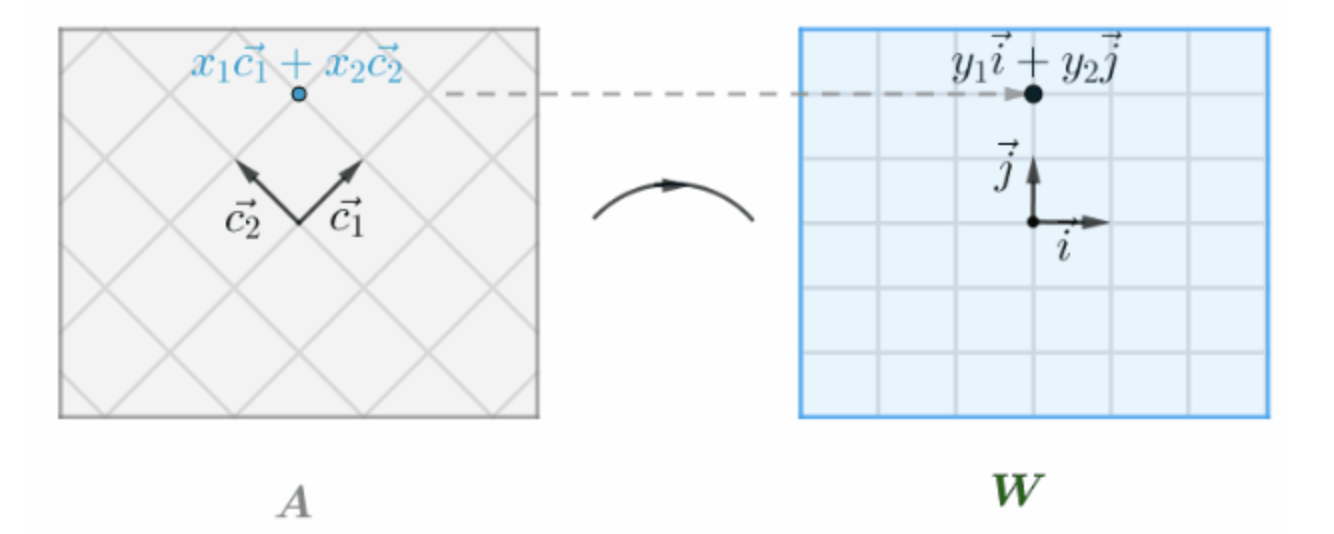
\includegraphics[width=.8\textwidth]{fig/UnderstandMatrixMultiplication_7.png}
\end{figure}

所以整体来说,就是\textbf{基改变,导致向量的坐标发生变化:}
\begin{figure}[H]
\centering
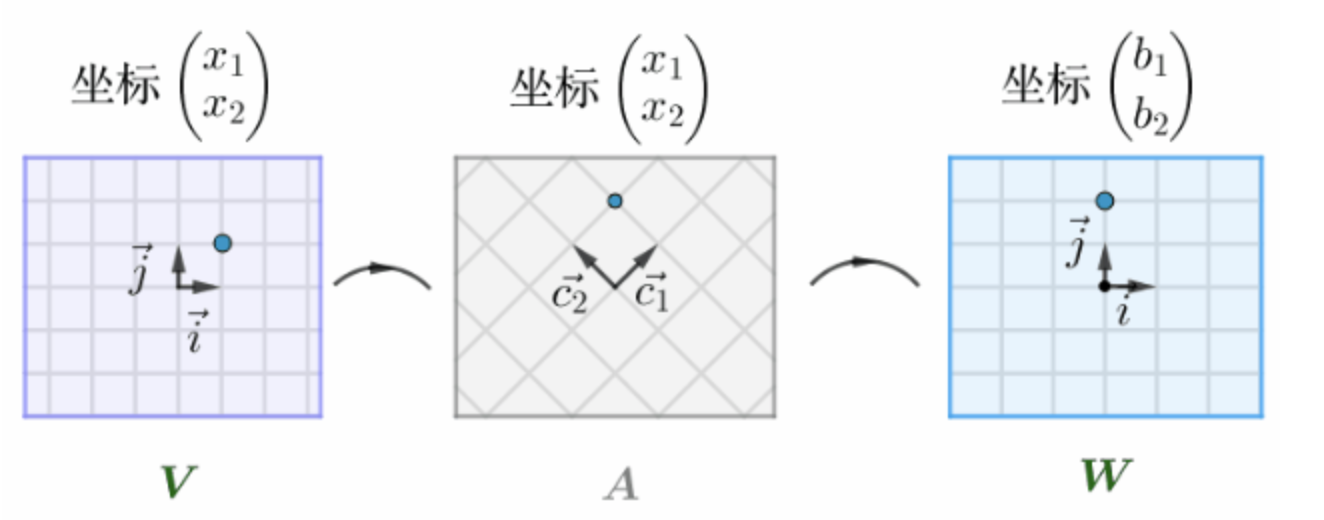
\includegraphics[width=.8\textwidth]{fig/UnderstandMatrixMultiplication_8.png}
\end{figure}

\subsection{复合函数和乘法交换律}
通过$G$把$\vec{x}$映射到$G(\vec{x})$,再通过$F$把$G(\vec{x})$映射到$\vec{y}$,矩阵的乘法$FG$可以如下图所示:
\begin{figure}[H]
\centering
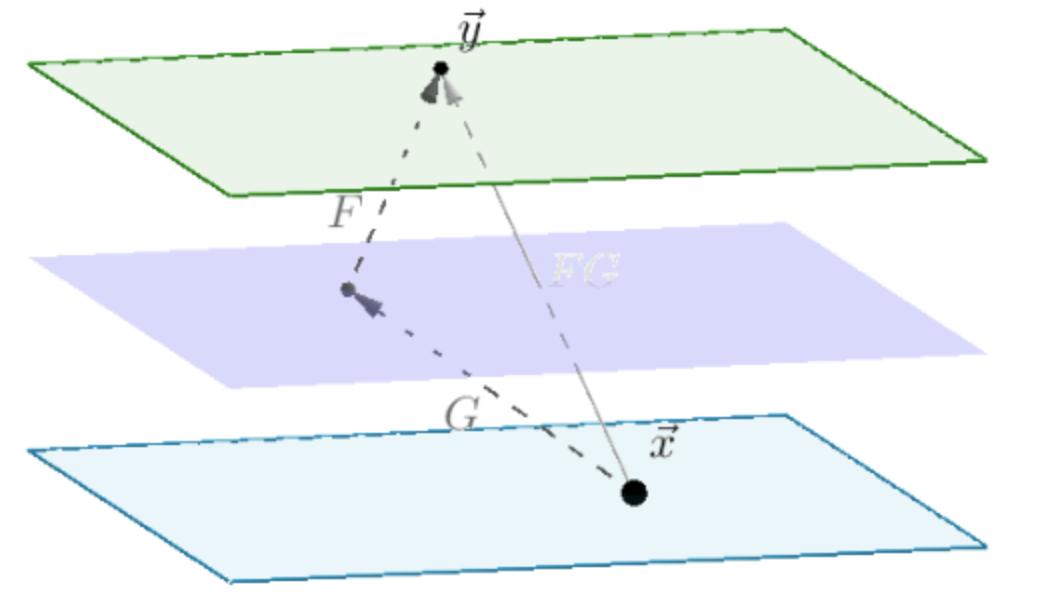
\includegraphics[width=.3\textwidth]{fig/UnderstandMatrixMultiplication_9.png}
\end{figure}

所以\textbf{矩阵乘法 $FG$实际上就是复合函数:
$FG \rightarrow F(G)$}

而函数一般是不满足交换律的,比如:
$f(x)=sin(x), g(x)=x^2$
那么:
$f(g(x))=sin(x^2)\ne g(f(x))=sin^2(x)$
那么矩阵乘法不满足交换律也很好理解了。

\textbf{即从复合函数的角度看(矩阵乘法就是复合函数),矩阵乘法不满足交换律是显然的。}

\subsection{从不同角度理解矩阵}
给定矩阵$A = \begin{bmatrix}
    a & b\\ c & d
\end{bmatrix}$,可以有不同的理解:
\subsubsection{从”图形“的角度理解}
将 $A$ 理解成以 $\vec{c_1} = \begin{bmatrix}a\\c\end{bmatrix},\vec{c_2} = \begin{bmatrix}b\\d\end{bmatrix}$为基张成的“\textbf{元平行四边形}”,此时$A$的行列式$det(A)$就表示以$c_1,c_2$张成的平行四边形的面积;同理,如果$A$是$3\times3$的,则$det(A)$代表平行六面体的体积;

\subsubsection{从线性变换的角度理解}
将 $A$ 理解成线性变换;单独看$A$,可以理解成对标准基进行了线性变换(如图);将$A$作用在向量$\vec{x}$上表示对向量 $\vec{x}$ 进行了线性变换,此时 $A\vec{x}$ 更应该写成 $A(\vec{x})$;如果记$\vec{x'} = A\vec{x}$,其中$x$的基为$\vec{i}, \vec{j}$,$x'$的基为$\vec{i'}, \vec{j'}$,那么矩阵$A$实际上是改变了基,通过$A$把$\vec{i}\rightarrow\vec{i'},\vec{j}\rightarrow\vec{j'}$,或者说矩阵$A$的列就是变换后的$\vec{i'}, \vec{j'}$;
\begin{figure}[H]
    \centering
    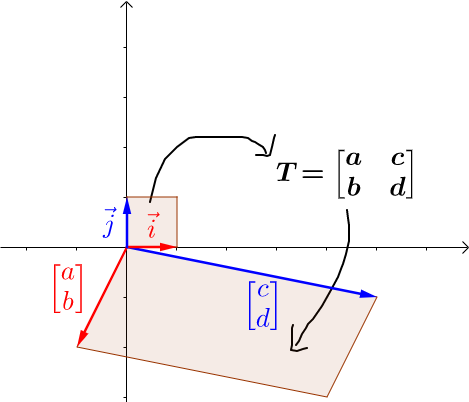
\includegraphics[width=.3\textwidth]{fig/UnderstandDeterminant_4.png}
\end{figure}

\subsubsection{从”运动“的角度理解}
将 $A$ 所代表的线性变换进一步理解成一种“运动”((广义的运动);对于运动而言,最重要的当然就是运动的
速度和方向,那么:
\begin{itemize}
\setlength{\itemsep}{0pt}
\setlength{\parsep}{0pt}
\setlength{\parskip}{0pt}
    \item 特征值就是运动的速度
    \item 特征向量就是运动的方向
\end{itemize}

\subsubsection{小结\cite{Fantastic_Matrix_1}}
\textbf{坐标系}是由\textbf{线性无关的向量}放在一起构成的,只是表示成\textbf{矩阵}的形式而已,而我们将常用的是 把\textbf{矩阵看成运动(线性代数里常称为变换)的描述},用乘法来施加,即\textbf{矩阵本身描述了一个坐标系,矩阵与矩阵的乘法描述了一个运动}。

换句话说:\textbf{如果矩阵仅仅自己出现,那么他描述了一个坐标系,如果他和另一个矩阵或向量同时出现,而且做乘法运算,那么它表示运动!}。

\subsection{矩阵与方程组\cite{Fantastic_Matrix_1}}
当解一个方程组的时候,我们知道,方程组的解只与系数有关。于是,将系数提取出来,放在一起,就构成了矩阵,而矩阵的行变换就 相当于解方程时的加减消元过程(也叫高斯消元法)。

下面我们从方程组解的几何意义来解释方程组 $Ax=b$ 的意义:
\begin{itemize}
\setlength{\itemsep}{0pt}
\setlength{\parsep}{0pt}
\setlength{\parskip}{0pt}
    \item 方程组有解可以理解成空间几何图形有公共交点或者交线(高维度时还可能出现 “交面”等情况)
    \item 方程组有解就说明 $b$ 这个向量能用 $A$ 的列向量线性表示,也可以说 $b$ 这个向量在 $A$ 的列向量所构成的空间中;因为我们可以将矩阵 $A_{n\times m}$ 写成这样列向量的表示形式:$A = [\vec{a_1}, \vec{a_2}, \cdots, \vec{a_n}]$,于是,方程就变成了$x_1\vec{a_1} + x_2\vec{a_2} + \cdots + x_n\vec{a_n}= b$,也就是说,如果一个方程组有解,就说明 $b$ 这个向量能用 
    $A$ 的列向量线性表示,也可以说 $b$ 这个向量在 $A$ 的列向量所构成的空间中。
\end{itemize}

举一个例子,对于方程组$\begin{cases}
2x-y=1 \\ x+y=5
\end{cases}$的几何意义如下:
\begin{figure}[H]
\centering
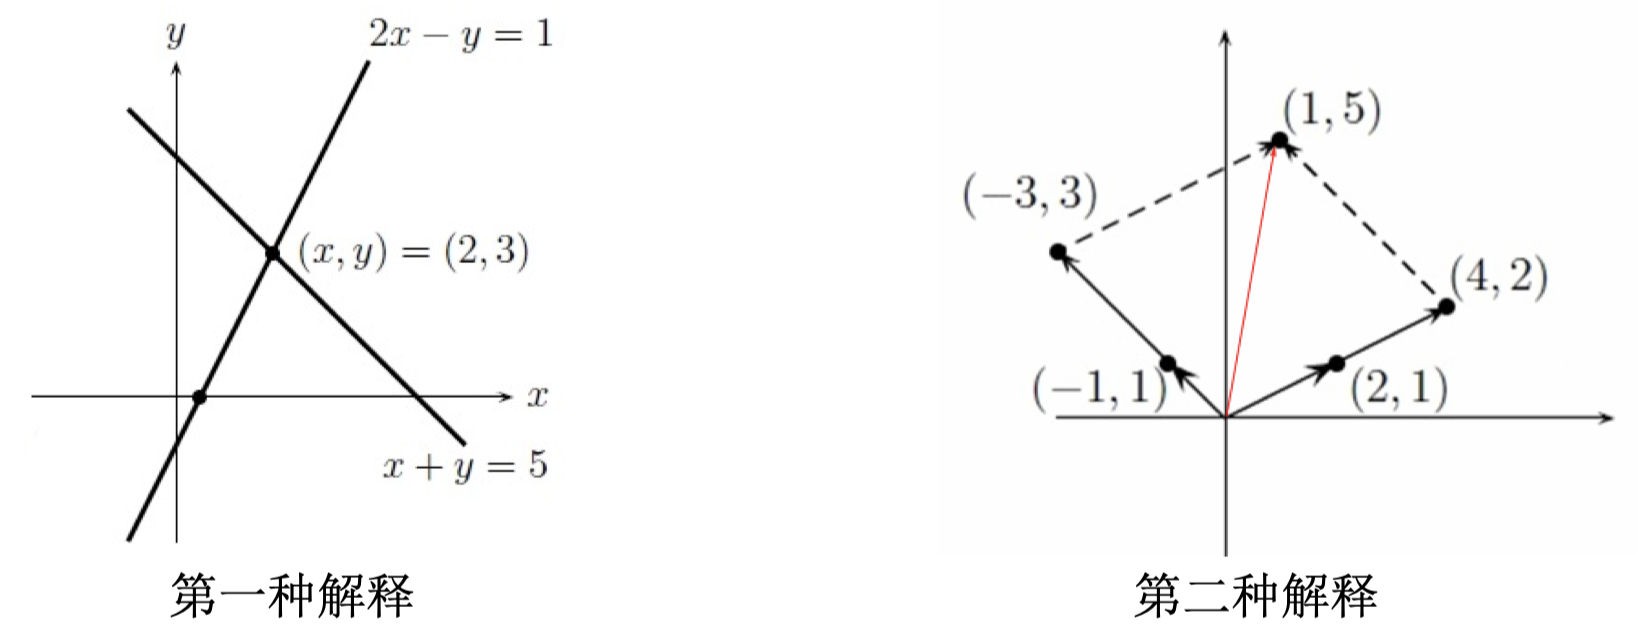
\includegraphics[width=.5\textwidth]{fig/FantasticMatrix_Season_1_1.png} 
\end{figure}

那么,无穷解和无解怎么理解呢?

对于第一种解释,无穷解代表有公共相交部分,但是最终形成的不是一个点,而是线或者面或者更高维的东西,而无解代表着没有公共相交的部分。

对于第二种解释,无穷解表示矩阵 $A$中的列向量线性相关,所以导致表示方式不唯一。而无解则表示矩阵 $A$ 中的列向量和 $b$ 不在同一个“次元”里,或者说不在一个空间里。如果 $A$ 的列向量和 $b$ 在同一个空间里,那么就需要 $A$ 的维数和$[A,b]$的维数相同。我们知道,矩阵的秩表示向量构成的空间的维数,于是我们知道 $r(A)$应该等于 $r([A,b])$,

\section{理解线性变换和仿射变换\cite{How_To_Understand_Affine_Transformation}}
\subsection{线性变换的要点}
线性变换的几何直观有三个要点:
\begin{itemize}
\setlength{\itemsep}{0pt}
\setlength{\parsep}{0pt}
\setlength{\parskip}{0pt}
    \item 变换前是直线的,变换后依然是直线
    \item 直线比例保持不变
    \item \textbf{变换前是原点的,变换后依然是原点}
\end{itemize}

比如旋转:对于以原点为中心的正方形,无论怎么旋转,之前的边是直线,之后的边仍然是直线;之前和之后的边长比例保持1:1;之前中心在原点,之后中心仍然在原点;比如推移:把正方形推移一下(变成平行四边形),直线还是直线;比例还是原来的比例;原点还是原点;比如旋转加推移,仍然保持上面三个性质不变。

\subsection{从线性函数到线性变换}
\subsubsection{线性函数与线性变换的关系}
直观地讲,函数就是把$x$轴上的点映射到曲线上。比如函数函数$y=sin(x)$,把$x$轴上的点映射到了正弦曲线上);还有的函数,比如$y=x$,是把$x$轴上的点映射到直线上,我们称为线性函数;

线性函数其实就是线性变换,为了看起来更像是线性变换,我换一种标记法。

比如对于$y=x$,我们可以认为是把$(a,0)$点映射到$(0,a)$点,我们称为线性变换$T$,记作:
$$
T:(a,0) \rightarrow (0,a), a \in \mathbb{R}, b \in \mathbb{R}
$$

矩阵的形式很显然如下:
$$
\begin{pmatrix}
0 \\ a
\end{pmatrix}
= \begin{pmatrix}
0 & 1 \\1 & 0 \\
\end{pmatrix}
\begin{pmatrix}
a \\ 0
\end{pmatrix}
$$

这样做最直接的好处是,\textbf{我们可以轻易的摆脱$x$轴的限制。}

\textbf{只要替换$(a,0)$为平面内所有的点$(a,b)$,我们就可以对整个平面做变换},该线性变换记作:
$$
T:(a,b) \rightarrow (b,a)
$$

进而可以写作矩阵的形式:
$$
\begin{pmatrix}
a \\ b
\end{pmatrix}
= \begin{pmatrix}
0 & 1 \\1 & 0 \\
\end{pmatrix}
\begin{pmatrix}
a \\ b
\end{pmatrix}
$$

也就是说整个平面的点都可以被变换。

使用线性代数的记号,有:
$$
\vec{x} = \begin{pmatrix}
a \\ b
\end{pmatrix} \quad
\vec{y} = \begin{pmatrix}
b \\ a
\end{pmatrix} \quad
A = \begin{pmatrix}
1&0 \\ 0&1
\end{pmatrix}
$$

即:
$$
\vec{y} = A\vec{x}
$$

进一步,既然$\vec{x},\vec{y}$都是平面上的点,我们可以认为:
\begin{center}
\textbf{线性变换通过矩阵$A$来表示}
\end{center}

而$y=x$只不过是这个 $A$ 的一种特殊情况。

\subsubsection{矩阵$A$与基}
因为 $y=x$ 是基于直角坐标系的,通过这个转换:
$$
y = x \rightarrow A = \begin{pmatrix}
1&0 \\ 0&1
\end{pmatrix}
$$

得到的$A$也是基于直角坐标系的。只是在线性变换中,我们不称为直角坐标系,我们叫做\textbf{标准正交基}。

标准正交基是:
$$
\vec{i} = \begin{pmatrix}1\\0\end{pmatrix}, \vec{j} = \begin{pmatrix}0\\1\end{pmatrix}
$$

它们所张成的线性空间如下:
\begin{figure}[H]
\centering
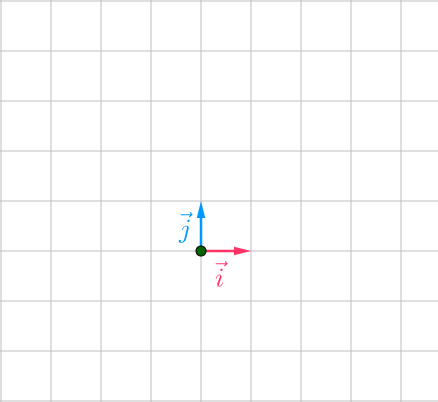
\includegraphics[width=.3\textwidth]{fig/UnderstandSimilarMatrix_2.png} 
\end{figure}

$A$在此基下,完成了镜面反转这个线性变换。

因此,让我们补完之前的结论:
\begin{center}
\textbf{线性变换通过}\textcolor{red}{指定基下的}{矩阵}A\textbf{来表示}
\end{center}


\subsection{线性变换的描述方法}
\subsubsection{用代数方式描述线性变换}
比如给定一个点$A$,它的坐标为:$(a,b)$;

我们也可以把它看做一个矢量和点以示区别,表示为矩阵:$\vec{A} = \begin{bmatrix}a \\ b\end{bmatrix}$;

用旋转矩阵
$$
T_{rotate}=\begin{bmatrix}cos(\theta)&-sin(\theta)\\sin(\theta)&cos(\theta)\end{bmatrix}
$$

与 $\vec{A}$ 进行矩阵乘法:
$$
T_{rotate}\vec{A} = \vec{A'}
$$
其中 $\vec{A} = a\vec{i} + b\vec{j}$,$\vec{A'} = a\vec{i'} + b\vec{j'}$

对正方形的每个点都运用 $T_{rotate}$ 就完成了旋转。所以实际上$T_{rotate}$是\textcolor{red}{改变了基},通过$T_{rotate}$对基进行了变换:$\vec{i} \rightarrow \vec{i'}, \vec{j} \rightarrow \vec{j'}$

详细点说,实际上,\textbf{矩阵的列其实就是变换后的$\vec{i'} \vec{j'}$},这就是矩阵的真正含义。

即对于旋转矩阵:
$$
T_{rotate}=\begin{bmatrix}cos(\theta)&-sin(\theta)\\sin(\theta)&cos(\theta)\end{bmatrix} \quad \Rightarrow \quad 
\vec{i'} = \begin{bmatrix}
cos(\theta) \\ sin(\theta)\end{bmatrix} \quad \vec{j'} = \begin{bmatrix}
\sin(\theta) \\cos(\theta)\end{bmatrix}
$$

我们只需要旋转基,就可以完成正方形的旋转。

\textbf{总结下来,线性变换是通过矩阵乘法来实现的;换句话说,矩阵变换的其实是基。}

\begin{framed}  
%\verb|\documentstyle[ifthen,12pt,titlepage]{article}|
\small{
\textbf{旋转矩阵的推导}

设点$(x,y)$离坐标原点距离$r$,与$x$轴夹角$\theta_0$ ,将点绕原点逆时针旋转$\theta$ ,旋转之后点的坐标为$(x',y')$。显然$(x',y')$ 与原点距离不变,仍然为$r$。
\begin{figure}[H]
\centering
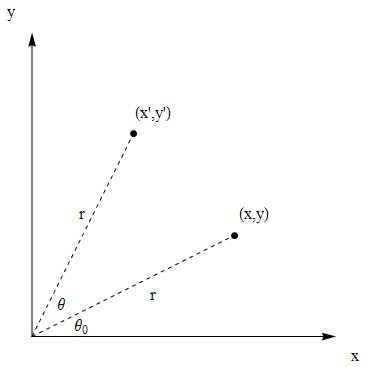
\includegraphics[width=.3\textwidth]{fig/UnderstandRotateMatrix.jpg}
\end{figure}

显然如下关系成立:
$$
\frac{x'}{r} = \cos{(\theta_0+\theta)} = \cos{\theta_0}\cos{\theta} - \sin{\theta_0}\sin{\theta} = \frac{x}{r}\cos{\theta} - \frac{y}{r}\sin{\theta}
$$
$$
\frac{y'}{r} = \sin{(\theta_0+\theta)} = \sin{\theta_0}\cos{\theta} - \cos{\theta_0}\sin{\theta} = \frac{y}{r}\cos{\theta} + \frac{x}{r}\sin{\theta}
$$

整理得到:
$$
x' = x\cos{\theta} - y\sin{\theta}
$$
$$
y' = x\sin{\theta} + y\cos{\theta}
$$

把上面这两个方程写成矩阵形式即可得到旋转矩阵的表达式:
$$
\begin{bmatrix}
x'\\y'
\end{bmatrix} = 
\begin{bmatrix}
\cos{\theta} & -\sin{\theta} \\
\sin{\theta} & \cos{\theta}
\end{bmatrix}
\begin{bmatrix}
x\\y
\end{bmatrix}
$$
}
\end{framed}

\subsection{仿射变换}
仿射变换从几何直观只有两个要点:
\begin{itemize}
    \item 变换前是直线的,变换后依然是直线
    \item 直线比例保持不变
\end{itemize}

少了原点保持不变这一条。比如允许平移:平移后,直线还是直线,比例还是那个比例,但是原点却发生了变化。

\textbf{因此,平移不再是线性变化了,而是仿射变化。}

\subsubsection{用代数方式描述仿射变换}
线性变换是通过矩阵乘法来实现的,仿射变换不能光通过矩阵乘法来实现,还得有加法。

仿射变换表示为:
$$
\vec{y} = A\vec{x} + b
$$

\subsection{通过线性变换来完成仿射变换}
将仿射变换的方程式改写下,可以发现仿射变换和线性变换的关系:
$$
\vec{y} = A\vec{x} + b \Rightarrow 
\begin{bmatrix}
    \vec{y}\\1
\end{bmatrix} = 
\begin{bmatrix}
    A & \vec{b}\\0 & 1
\end{bmatrix}
\begin{bmatrix}
    \vec{x}\\1
\end{bmatrix}
$$

也就是说,\textcolor{red}{增加一个维度后,就可以在高维度通过线性变换来完成低维度的仿射变换。}

举个例子:
\begin{figure}[H]
    \centering
    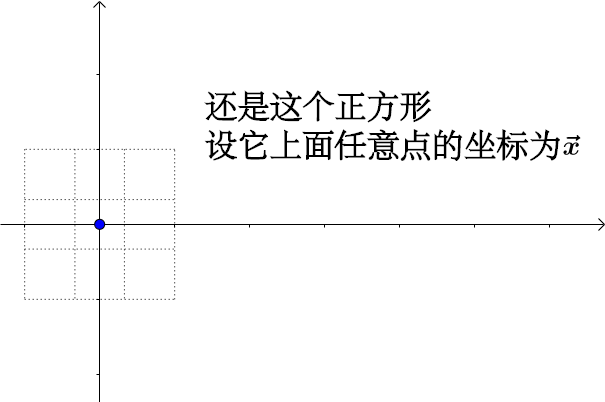
\includegraphics[width=.5\textwidth]{fig/UnderstandAffineTransformation_1.png}
\end{figure}
\begin{figure}[H]
    \centering
    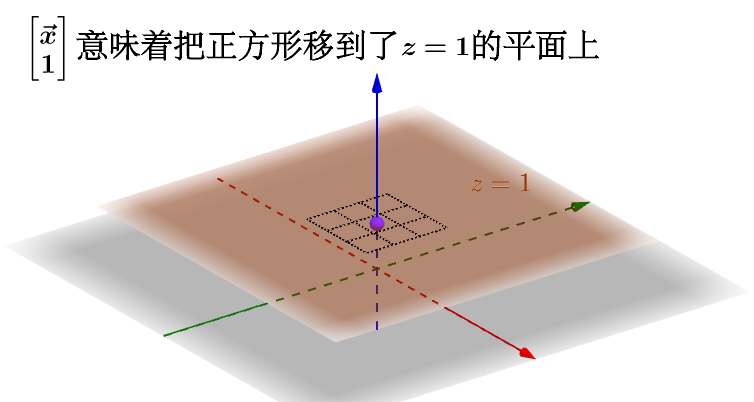
\includegraphics[width=.5\textwidth]{fig/UnderstandAffineTransformation_2.png}
\end{figure}
\begin{figure}[H]
    \centering
    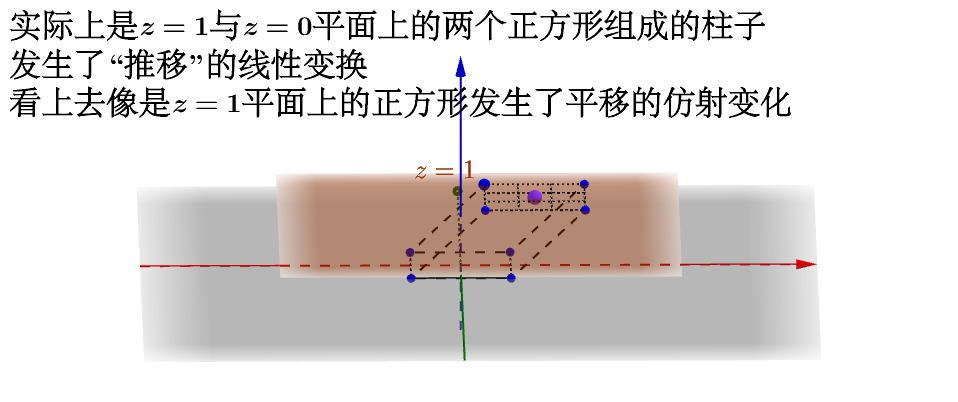
\includegraphics[width=.5\textwidth]{fig/UnderstandAffineTransformation_3.png}
\end{figure}
\begin{figure}[H]
    \centering
    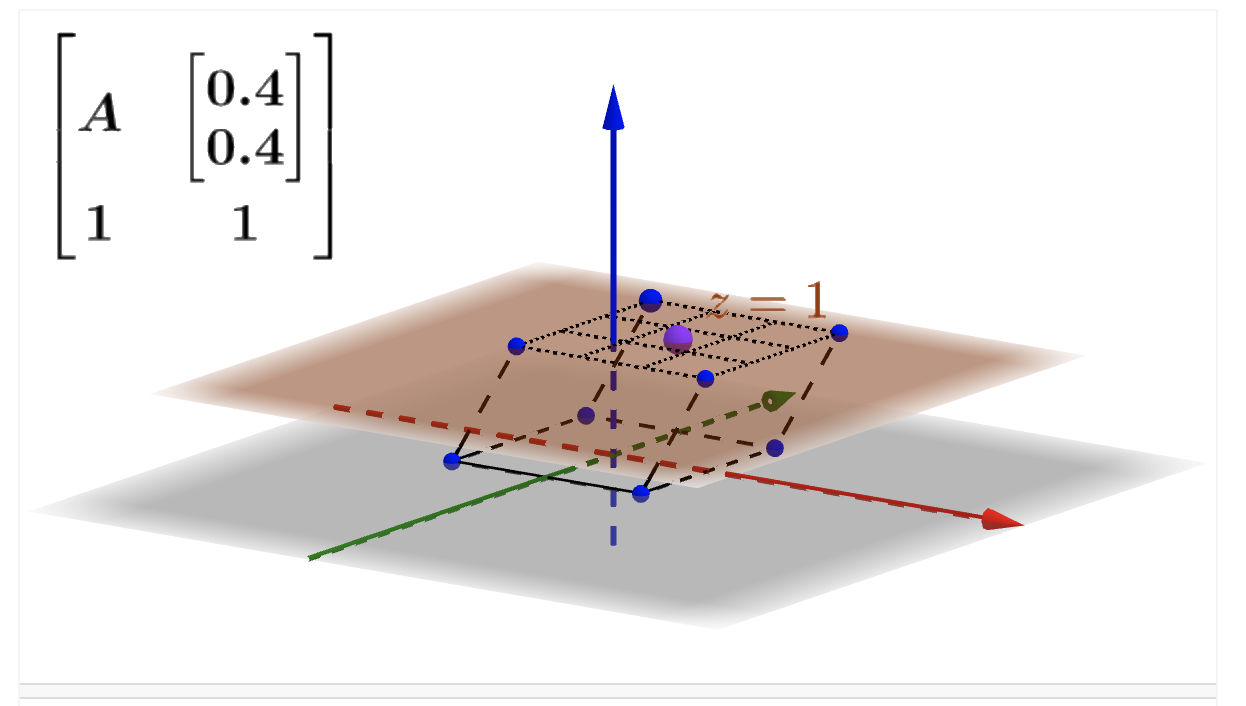
\includegraphics[width=.5\textwidth]{fig/UnderstandAffineTransformation_4.png}
\end{figure}
\begin{figure}[H]
    \centering
    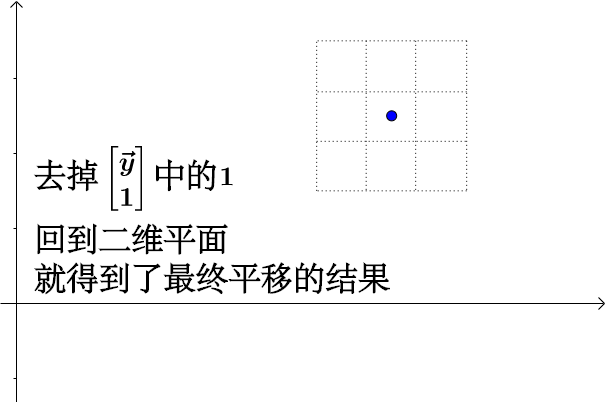
\includegraphics[width=.5\textwidth]{fig/UnderstandAffineTransformation_5.png}
\end{figure}

回忆一下计算机图形学:描述三维空间中的物体只需要三维向量,但是计算机图形学变换矩阵都是$4\times 4$的;这是因为,在计算机图形学里应用的图形变换,实际上是 在仿射空间而不是向量空间中进行的。所以计算机 图形学的生存空间实际上是仿射空间,而仿射变换的矩阵表示就是$4\times 4$ 的\cite{Fantastic_Matrix_1}。

\section{理解行列式\cite{How_To_Understand_Determinant}}
\subsection{行列式的来历和本质}
人们为了解线性方程组,最终总结出了行列式。\textcolor{red}{行列式的本质是线性变换的伸缩因子。}

\subsection{行列式的本质是线性变换的伸缩因子}
我们还是拿旋转矩阵来举例子:
$$
T_{rotate}=\begin{bmatrix}cos(\theta)&-sin(\theta)\\sin(\theta)&cos(\theta)\end{bmatrix} \Rightarrow |T_{rotate}| = \begin{vmatrix}cos(\theta)&-sin(\theta)\\sin(\theta)&cos(\theta)\end{vmatrix} = \cos^2(\theta) + \sin^2(\theta) = 1
$$

$T_{rotate}$ 的行列式恒等于1,意味着旋转不会改变面积。

同理,对于缩放矩阵:
$$
T_{scale} = \begin{bmatrix}a&0\\0&b\end{bmatrix}
$$
$$
T_{scale}\vec{X} = \begin{bmatrix}a&0\\0&b\end{bmatrix}
\begin{bmatrix}x_1\\x_2\end{bmatrix} = 
x_1\begin{bmatrix}a\\0\end{bmatrix} + 
x_2\begin{bmatrix}0\\b\end{bmatrix}
$$
$$
|T_{scale}| = \begin{vmatrix}a&0\\0&b\end{vmatrix} = ab
$$

变换后,$\vec{i}$对应的坐标会缩放为$a$倍,$\vec{j}$对应的坐标会缩放为$b$倍,面积会缩放为原来的$ab$倍;

掌握了行列式是线性变换的伸缩因子这一点之后,我们就很容易理解各种行列式的值与线性变换的关系。

\subsection{行列式大小对变换的影响}
\subsubsection{行列式$>0$}
\begin{itemize}
    \item 行列式$>1$,对于图形有放大的作用
    \item 行列式$=1$,图形的大小不会变换
    \item $0<$行列式$<1$,对于图形有缩小的作用
\end{itemize}

\subsubsection{行列式$=0$}
\textbf{行列式等于0,有一个重要的结论是,矩阵不可逆。}

还是以旋转矩阵为例,通过旋转矩阵,逆时针旋转$45^\circ$,旋转矩阵为:
$$
T_{rotate}(45^\circ)=\begin{bmatrix}cos(45^\circ)&-sin(45^\circ)\\sin(45^\circ)&cos(45^\circ)\end{bmatrix}
$$

再通过另外一个旋转矩阵,顺时针旋转$45^\circ$,旋转矩阵为:
$$
T_{rotate}(-45^\circ)=\begin{bmatrix}cos(-45^\circ)&-sin(-45^\circ)\\sin(-45^\circ)&cos(-45^\circ)\end{bmatrix}
$$

两次旋转后,原图形看起来就像没有变换过一样,因此:$T_{rotate}(-45^\circ)$和$T_{rotate}(45^\circ) $ 互为逆矩阵。

有的线性变换是可逆的,有的不行,比如行列式=0这样的线性变换就是不可逆的。从图像上看,图形会缩成一点$\begin{bmatrix}0&0\\0&0\end{bmatrix}$,或者缩成一条直线$\begin{bmatrix}0&0\\0&1\end{bmatrix}$;没有矩阵可以把它们恢复成原来的样子。

\subsubsection{行列式$<0$}

原始图像是这样的:
\begin{figure}[H]
\centering
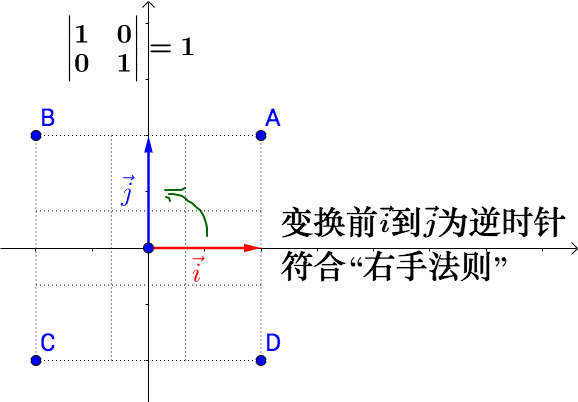
\includegraphics[width=.5\textwidth]{fig/UnderstandDeterminant_1.png}
\end{figure}

被行列式 $< 0$的矩阵线性变换后是这样的:
\begin{figure}[H]
\centering
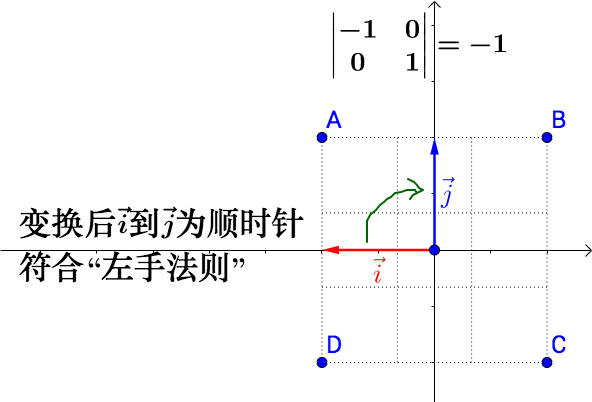
\includegraphics[width=.5\textwidth]{fig/UnderstandDeterminant_2.png}
\end{figure}

行列式 $< 0$其实就是改变了基的“左右手法则”

\subsection{推论}
知道了行列式的意义,我们就很容易知道,为什么
\begin{itemize}
    \item 矩阵乘法不满足交换律:$T_1T_2 \neq T_2T_1$:因为矩阵乘法相当于复合函数
    \item 但是:$det(T_1T_2) = det(T_2T_1)$:因为面积先缩放为$T_1$倍再缩放为$T_2$倍,与先缩放为$T_2$倍再缩放为$T_1$倍等价
\end{itemize}

同理,可以知道为什么
\begin{itemize}
    \item 二阶矩阵的行列式是\textbf{列}组成的平行四边形的\textbf{面积}(对单位正方形进行了缩放)
\begin{figure}[H]
    \centering
    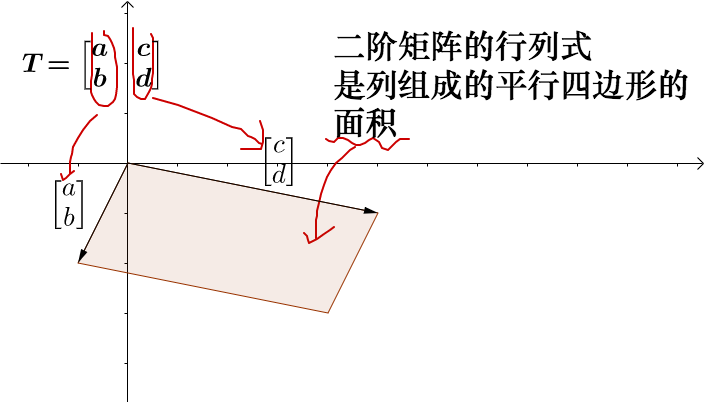
\includegraphics[width=.5\textwidth]{fig/UnderstandDeterminant_3.png}
\end{figure}
\begin{figure}[H]
    \centering
    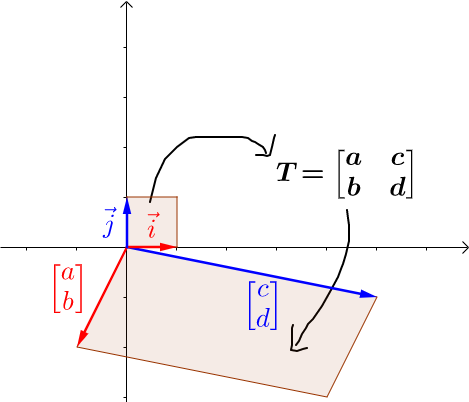
\includegraphics[width=.5\textwidth]{fig/UnderstandDeterminant_4.png}
\end{figure}  
    \item 三阶矩阵的行列式是\textbf{列}组成的平行六面体的\textbf{体积}(对单位正方体进行了缩放
\end{itemize}

\section{理解正交矩阵\cite{Fantastic_Matrix_1}}
\subsection{正交矩阵的定义}
如果:$AA^T=E$($E$为单位矩阵,$A^T$表示“矩阵$A$的转置矩阵”)或$A^TA=E$,则$n$阶实矩阵$A$称为正交矩阵。

\subsection{正交矩阵的性质}
\begin{itemize}
\setlength{\itemsep}{0pt}
\setlength{\parsep}{0pt}
\setlength{\parskip}{0pt}
    \item $A^T$是正交矩阵
    \item $A$的各行是单位向量且两两正交
    \item $A$的各列是单位向量且两两正交
    \item $|A|=1$或$-1$
    \item \textbf{正交矩阵的乘积仍是正交矩阵}
\end{itemize}

\begin{framed}  
%\verb|\documentstyle[ifthen,12pt,titlepage]{article}|
\small{
证明正交矩阵的乘积仍是正交矩阵。

假定$M,N$是正交矩阵,即:
$$
MM^T = MM^{-1} = E, NN^T = NN^{-1} = E
$$

那么:
$$
(MN)(MN)^T = (MN)(N^TM^T) = MNN^TM^T = MEM^T = E
$$

即$MN$ 仍是正交矩阵。
}
\end{framed}

\subsection{正交矩阵的直观理解}
正交矩阵是方块矩阵,行向量和列向量皆为正交的单位向量。

正交矩阵的定义“行向量和列向量皆为正交的单位向量”带来了另一个好处:\textbf{正交矩阵的转置就是正交矩阵的逆,比普通矩阵求逆矩阵简单多了}。即:
$$
MM^{-1} = MM^T = E
$$

举例证明上述结论:给定正交矩阵
$$
M = \begin{bmatrix}
\vec{x_1}, & \vec{x_2}, &\vec{x_3}
\end{bmatrix} = 
\begin{bmatrix}
\vec{y_1} \\ \vec{y_2} \\ \vec{y_3}
\end{bmatrix} = 
\begin{bmatrix}
x_{11} & x_{12} & x_{13} \\
x_{21} & x_{22} & x_{23} \\
x_{31} & x_{32} & x_{33} \\
\end{bmatrix}
$$

因为每行(每列)都是单位长度向量,所以每行点乘自己(每列点乘自己)的结果为1:
$$
\vec{x_i}\cdot\vec{x_i} = 1, \quad i = 1, 2, 3
$$
$$
\vec{y_i}\cdot\vec{y_i} = 1, \quad i = 1, 2, 3
$$

因为任意两行(两列)正交,所以就是两行(两列)点乘结果为0:
$$
\vec{x_i}\cdot\vec{x_j} = 0, \quad i \ne j
$$
$$
\vec{y_i}\cdot\vec{y_j} = 0, \quad i \ne j
$$

并且$M$的转置为:
$$
M^T = \begin{bmatrix}
\vec{x_1} \\ \vec{x_2} \\ \vec{x_3}
\end{bmatrix} = 
\begin{bmatrix}
\vec{y_1} & \vec{y_2} & \vec{y_3}
\end{bmatrix} = 
\begin{bmatrix}
x_{11} & x_{21} & x_{31} \\
x_{12} & x_{22} & x_{32} \\
x_{13} & x_{23} & x_{33} \\
\end{bmatrix}
$$

所以,有:
$$
MM^T = \begin{bmatrix}
\vec{y_1}\cdot\vec{y_1} & \vec{y_1}\cdot\vec{y_2} & \vec{y_1}\cdot\vec{y_3} \\
\vec{y_2}\cdot\vec{y_1} & \vec{y_2}\cdot\vec{y_2} & \vec{y_2}\cdot\vec{y_3} \\
\vec{y_3}\cdot\vec{y_1} & \vec{y_3}\cdot\vec{y_2} & \vec{y_3}\cdot\vec{y_3} \\
\end{bmatrix} = 
\begin{bmatrix}
1 & 0 & 0 \\ 0 & 1 & 0 \\ 0 & 0 & 1
\end{bmatrix}
$$

不难验证,旋转矩阵
$$
T = \begin{bmatrix}
\cos\theta & -\sin\theta \\ \sin\theta & \cos\theta
\end{bmatrix}
$$
也是正交矩阵,从而有:旋转矩阵的逆矩阵是它的转置矩阵,即:
$$
TT^{-1} = TT^T = E
$$

一个矩阵是旋转矩阵,当且仅当它是正交矩阵并且它的行列式是单位1。

\textbf{正交矩阵的行列式是 $\pm 1$;如果行列式是 $−1$,则它包含了一个反射而不是真旋转矩阵}。

对于旋转矩阵乘幂,我们可以知道,就是一直旋转,乘了几次就是旋转了几次。当好多个旋转矩阵(可以不同)连乘时,我们就能理解了,这是把一个向量沿着多个方向旋转 的叠加。

\section{理解矩阵的「秩」\cite{How_To_Understand_Rank_Of_Matrix}}
「秩」是图像经过矩阵变换之后的空间维度

「秩」是列空间的维度

\subsection{「秩」是图像经过矩阵变换之后的空间维度}
比如给定原始图像为以原点为中心的正方形,通过旋转矩阵$T_1=\begin{bmatrix}cos(\theta)&-sin(\theta)\\sin(\theta)&cos(\theta)\end{bmatrix}$进行变换,变换后的图像是旋转后的正方形(二维);因此,旋转矩阵的「秩」为2。

再通过矩阵$T_2=\begin{bmatrix}1&-1\\1&-1\end{bmatrix}$进行变换,变换后的图像是一根一维的直线;因此,该变换矩阵的「秩」为1(想象一下$T_2$的基,是长度相等方向相反的两个向量,是线性相关的)。

再通过矩阵$T_3=\begin{bmatrix}0&0\\0&0\end{bmatrix}$进行变换,变换后的图像是一个零维的点;因此,该变换矩阵的「秩」为0(想象一下$T_3$的基,是重合的两个原点)。

\subsection{「秩」是列空间的维度}
\subsubsection{列空间}
我们通过旋转矩阵来解释什么是列空间;给定旋转矩阵
$$
T_{rotate}=
\begin{bmatrix}
    cos(\theta) & -sin(\theta)\\
    sin(\theta) & cos(\theta)
\end{bmatrix}
$$

该旋转矩阵的列向量分别是$\vec{i}=\begin{bmatrix}cos(\theta)\\sin(\theta)\end{bmatrix}$和$\vec{j}=\begin{bmatrix}-sin(\theta)\\cos(\theta)\end{bmatrix}$这两个向量不在一条直线上,我们称其为线性无关。

通过改变$a,b$的值,可以用$a\vec{i} + b\vec{j}$来表示二维平面上的所有点。

所以,\textbf{列空间就是矩阵的列向量所能张成(即通过$a\vec{i} + b\vec{j}$来表示)的空间。}

\textbf{列空间的维度就是「秩」};旋转矩阵的列空间是二维的,所以「秩」就为2。

\subsubsection{矩阵的变换目标是列空间}
给定矢量$\vec{A} = \begin{bmatrix}a\\b\end{bmatrix}$,同时,矢量$\vec{A}$也可以表示为$a\vec{i}+b\vec{j}$,其中$\vec{i},\vec{j}$ 为基向量。用基来表示的原因是因为矩阵变换的其实是基。

举例子来看看,比如给定旋转矩阵 $T_{rotate}$ 作用在矢量 $\vec{A}$上,有:
$$
\vec{A'} = T_{rotate}\vec{A}
$$

其中,$\vec{A} = a\vec{i} + b\vec{j}$,$\vec{A'} = a\vec{i'} + b\vec{j'}$

所以实际上是$T_{rotate}$是\textcolor{red}{改变了基},通过 $T_{rotate}$把$\vec{i} \rightarrow \vec{i'}$,$\vec{j} \rightarrow \vec{j'}$。

如果要说详细点,实际上矩阵的列就是变换后的$\vec{i'},\vec{j'}$,这就是矩阵的真正含义。

所以:$\vec{A} = a\vec{i} + b\vec{j} \Rightarrow \vec{A'} = a\vec{i'} + b\vec{j'}$ 实际上是变换到了$T_{rotate}$的列空间。

\subsubsection{两种定义方式的联系}
用旋转矩阵对二维的正方形进行线性变换,实际上是一个二维空间到另外一个二维空间的变换:

比如对于旋转矩阵,图像从$\vec{i}$,$\vec{j}$张成的空间,变换到$\vec{i'}$,$\vec{j'}$张成的空间。因为都是二维,所以图像维度不变。

但是对于矩阵$\begin{bmatrix}1&-1\\1&-1\end{bmatrix}$他的列空间是一维的;因此,这个矩阵的「秩」就是1,用它对二维的正方形进行线性变换,实际上是一个二维空间到另外一个一维空间的变换(即二维正方形会被压缩到一维直线上);

同理,矩阵$\begin{bmatrix}0&0\\0&0\end{bmatrix}$他的列空间是一个点,所以它的「秩」就是0。

\subsection{关于严格性的一个问题}
上面说矩阵的「秩」是列空间的维度,这并非完全正确的。

列空间的维度准确来说,是「列秩」,行空间的维度是「行秩」,但是,还好有,「秩」=「列秩」=「行秩」是恒成立的。所以直接把「列秩」称为「秩」也不算错误。

\begin{framed}  
%\verb|\documentstyle[ifthen,12pt,titlepage]{article}|
\small{
了解了秩,就很容易回答下面的问题。

我们知道矩阵是做线性变换的,比如说一个$3\times2$的矩阵,
\begin{figure}[H]
    \centering
    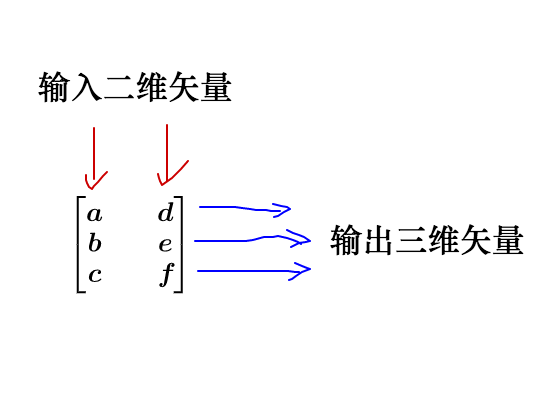
\includegraphics[width=.3\textwidth]{fig/UnderstandDeterminant_5.png}
\end{figure}  

从图像上看,平面上的一个矢量被一个$3\times2$的矩阵变换到了三维空间:
\begin{figure}[H]
    \centering
    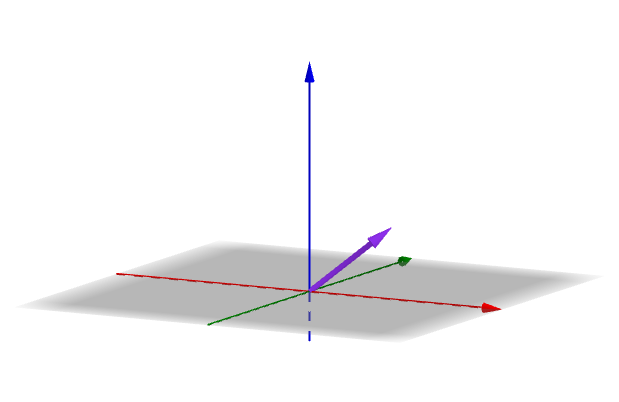
\includegraphics[width=.3\textwidth]{fig/UnderstandDeterminant_6.png}
\end{figure} 

那么,通过$3\times2$的矩阵能否把一个二维正方形变换为一个三维正方体呢?

答案是不行。三方的立方体需要存在于用三个正交的基张成的列空间中;如果把$3X2$的向量变换成 
$\begin{bmatrix}
a&d&0\\b&e&0\\c&f&0
\end{bmatrix}$;
可以看出来,它的第三个列空间是0维的,所以,用该矩阵进行线性变换后,只能将原向量变换到另一个二维的平面上,不能变换到一个三维的空间中。
}
\end{framed}

\subsection{理解行秩和列秩的关系\cite{Why_Rank_Of_Row_Column_Equal}}
TBD

\section{理解相似矩阵\cite{How_To_Understand_Similar_Matrix}}
相似矩阵的定义是:
设$A,B$都是$n$阶矩阵,若有可逆矩阵$P$,使:
$$
P^{-1}AP=B
$$
则称$B$是$A$的相似矩阵,或说$A$和$B$相似。

\subsection{通俗解释}
观看同样一部电影,坐在不同的位置,各自眼中看到的电影因为位置不同而有所不同(比如清晰度、角度),所以说,“第一排看到的电影”和“最后一排看到的电影”是“相似”的。

那么背后什么是不变的呢?是线性变换。

\subsection{坐标转换}
从数学角度上看,相似变换就是进行了坐标转换。

坐标转换是数学中的常用伎俩,目的是简化运算。比如常见的,把直角坐标系($xy$坐标系)的圆方程换元为极坐标($\rho\theta$坐标系)下:
$$
x^2 + y^2 = a^2 \Rightarrow \begin{cases}
\rho = a \\
\theta \in \mathbb{R}
\end{cases}
$$

图像也从左边变为了右边:
\begin{figure}[H]
    \centering
    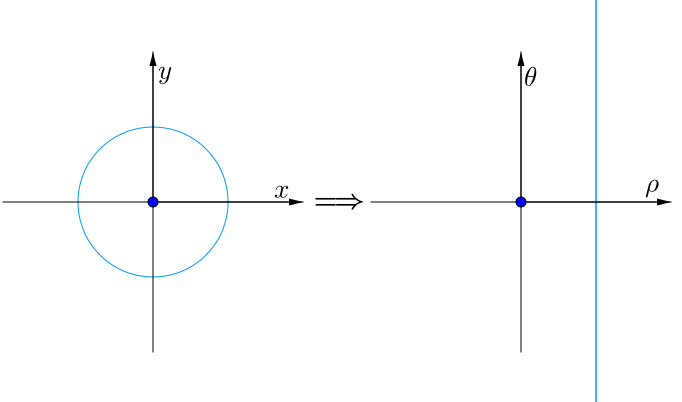
\includegraphics[width=.5\textwidth]{fig/UnderstandSimilarMatrix_1.png}
\end{figure} 

换元之后的代数式和图像都变简单了。相似变换也是这样的目的。

\subsection{相似矩阵}
回到开头给出看电影的例子,同一部“电影”,不同基“看到”的就是不同的矩阵,也就是说:

\begin{center}
\textbf{相同线性变换,}\textcolor{red}{不同基下的}\textbf{矩阵,称为相似矩阵}
\end{center}

那怎么得到不同基下的矩阵呢?让我们来看看变换的细节。

\subsubsection{变换的细节}
先上一张图,说明不同基下的矩阵的变换思路,这个图有点复杂,请参照之后的解释一起来看:
\begin{figure}[H]
    \centering
    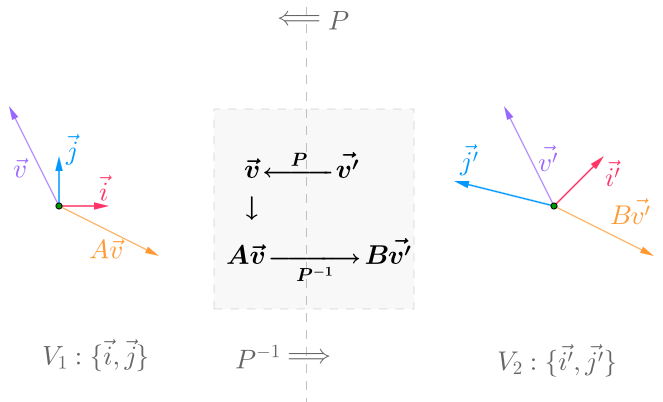
\includegraphics[width=.8\textwidth]{fig/UnderstandSimilarMatrix_3.png}
\end{figure} 

下面是对图的解释:
\begin{itemize}
    \item 有两个基:$V_1:\{\vec{i},\vec{j}\}$和$V_2:\{\vec{i'}, \vec{j}\}$
    \item $V_1 \rightarrow V_2$,可以通过 $P^{-1}$ 转换
    \item $V_2 \rightarrow V_1$,可以通过$P$ 转换
\end{itemize}

整个转换的核心,就是上图正中的文字,解释下:
\begin{itemize}
    \item $\vec{v'}$ 是$V_2$下的点
    \item $\vec{v'}$ 通过 $P$ 变换为 $V_1$ 下的点,即$P\vec{v'}$
    \item 在 $V_1$ 下,通过矩阵 $A$ 完成线性变换,即$AP\vec{v'}$
    \item 通过 $P^{-1}$ 重新变回$V_2$下的点,即$P^{-1}AP\vec{v'}$
\end{itemize}

综上,我们可以有:
$$
B\vec{v'} = P^{-1}AP\vec{v'}
$$

那么$B$和$A$互为相似矩阵。

\textcolor{red}{注意,这里的 $P$ 只进行了坐标基之间的变换,\textbf{所以$det(P) = \pm 1$};但是 $A$ 是线性变换,\textbf{所以可以有$det(A) \ne \pm 1$}。}

\subsubsection{对角矩阵}
那么为什么我们需要相似矩阵呢?

比如这个矩阵$A$:
$$
A = \begin{pmatrix}2&-1\\-1&2\end{pmatrix}
$$

可以这样分解:
$$
B = P^{-1}AP = \begin{pmatrix}3&0\\0&1\end{pmatrix}
$$

其中 $P = P^{-1} = \begin{pmatrix}
-\frac{\sqrt{2}}{2}&\frac{\sqrt{2}}{2}\\
\frac{\sqrt{2}}{2}&\frac{\sqrt{2}}{2}
\end{pmatrix}$

$B$就是对角矩阵,看上去就很清爽,所以说相似变换就是坐标转换,转换到一个更方便计算的简单坐标系。

\section{理解二次型\cite{How_To_Understand_Quadratic_Form}}
二次型就是通过矩阵研究二次函数。

通过矩阵来研究二次函数(方程),这就是线性代数中二次型的重点。

\subsection{二次函数(方程)的特点}
最简单的一元二次函数就是:$y = x^2$,给它增加一次项和常数项:$y = x^2 + px + q$ 不会改变它的形状(只会改变对称轴的位置和在 $y$ 轴的截距)

再看二元二次方程:$x^2 + xy + y^2 = 1$
\begin{figure}[H]
    \centering
    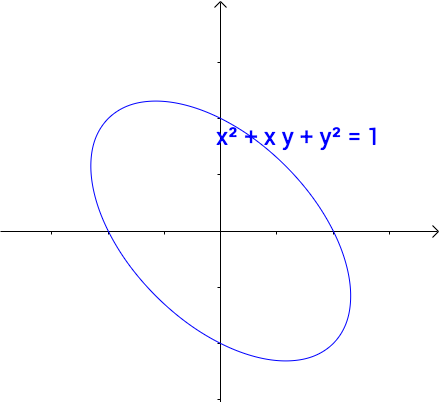
\includegraphics[width=.3\textwidth]{fig/UnderstandQuadraticForm_1.png}
\end{figure} 

给它增加一次项也不会改变形状$x^2 + xy + y^2 + 0.3x = 1$,只是看上去有些伸缩:
\begin{figure}[H]
    \centering
    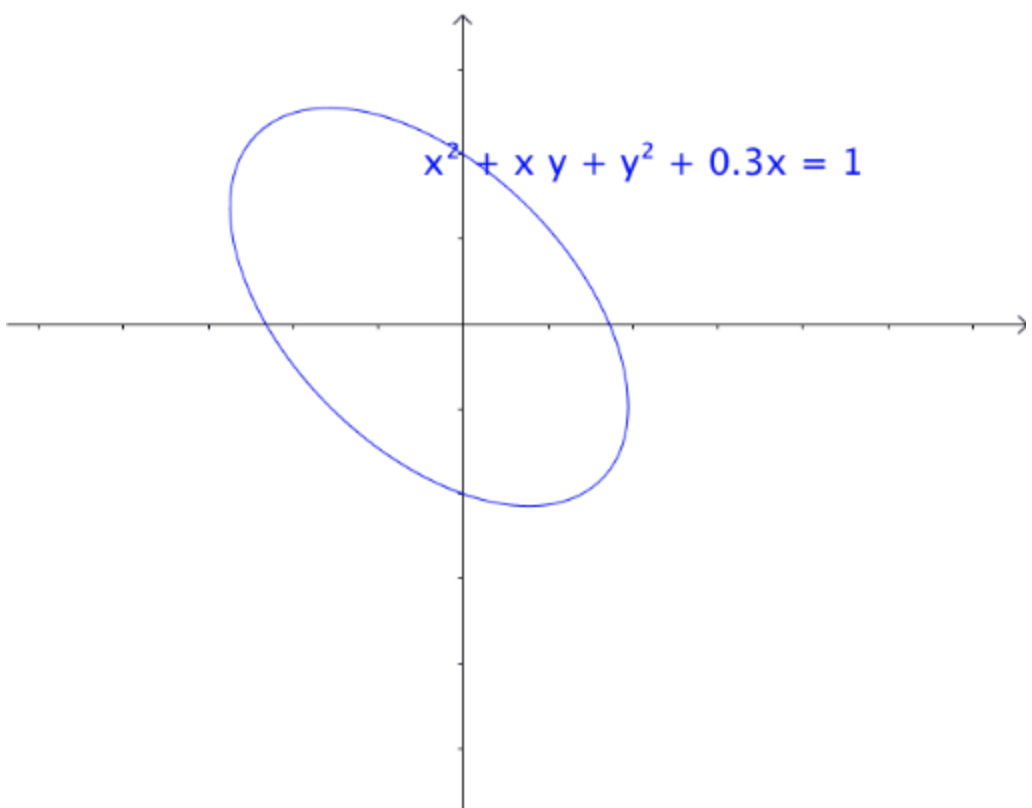
\includegraphics[width=.3\textwidth]{fig/UnderstandQuadraticForm_2.png}
\end{figure} 

所以,对于二次函数或者二次方程,\textbf{二次部分是主要部分,往往研究二次这部分就够了}。

\subsection{通过矩阵来研究二次方程}
因为二次函数(方程)的二次部分最重要,为了方便研究,我们把含有$n$个变量的二次齐次函数:
\begin{align*}
f(x_1, x_2, \cdots, x_n) &= a_{11}x_1^2 + a_{22}x_2^2 + \cdots + a_{nn}x_n^2 \\
 &+ 2a_{12}x_1x_2 + 2a_{13}x_1x_3 + \cdots + 2a_{n-1,n}x_{n-1}x
\end{align*}
或者二次齐次方程称为二次型。

\subsubsection{二次型矩阵}
实际上我们可以通过矩阵来表示二次型:
$$
x^2 - xy + y^2 = 1 \Rightarrow 
\begin{bmatrix}x & y\end{bmatrix}
\begin{bmatrix}1&-0.5\\-0.5&1\end{bmatrix}
\begin{bmatrix}x \\ y\end{bmatrix} = 1
$$

其中,$\left[\begin{smallmatrix}1&-0.5\\-0.5&1\end{smallmatrix}\right]$就是二次型。

更一般的:
$$
ax^2 + 2bxy + cy^2 = 1\Rightarrow 
\begin{bmatrix}x & y\end{bmatrix}
\textcolor{red}{\begin{bmatrix}a&b\\b&c\end{bmatrix}}
\begin{bmatrix}x \\ y\end{bmatrix} = 1
$$

可以写成更线代的形式:
$$
\left.
\begin{matrix}
\begin{bmatrix}x & y\end{bmatrix}
\begin{bmatrix}a&b\\b&c\end{bmatrix}
\begin{bmatrix}x \\ y\end{bmatrix} = 1 \\
\\
X =  \begin{bmatrix}x \\ y\end{bmatrix}\\
\\
A = \begin{bmatrix}a&b\\b&c\end{bmatrix} \\
\end{matrix}
\right\}
\Rightarrow X^TAX
$$

所以有下面一一对应的关系:
\begin{center}
\textbf{对称矩阵$\Longleftrightarrow$二次型矩阵$\Longleftrightarrow$二次型矩阵}
\end{center}

在线代里面,就是通过一个对称矩阵,去研究某个二次型。

\subsubsection{通过矩阵来研究有什么好处}
\textbf{圆锥曲线}

我们来看下,这是一个圆:
\begin{figure}[H]
    \centering
    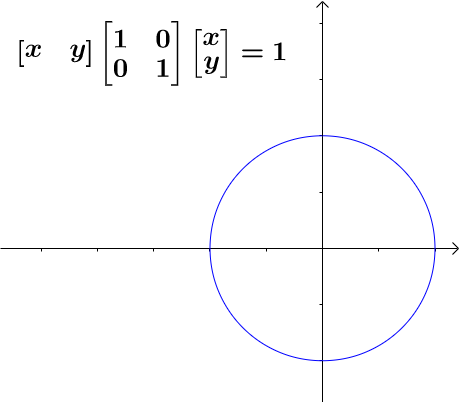
\includegraphics[width=.3\textwidth]{fig/UnderstandQuadraticForm_3.png}
\end{figure} 

然后看改变一下二次型矩阵:
\begin{figure}[H]
    \centering
    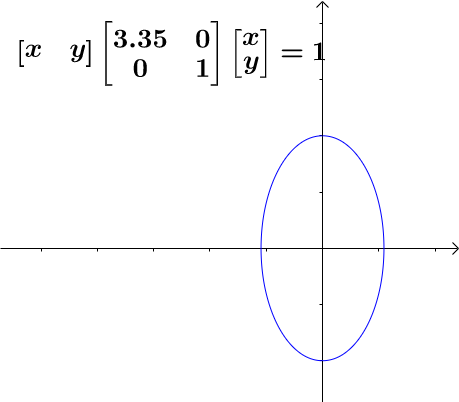
\includegraphics[width=.3\textwidth]{fig/UnderstandQuadraticForm_4.png}
\end{figure} 

所以原来椭圆和圆之间是线性关系(通过矩阵变换就可以从圆变为椭圆)。

继续:
\begin{figure}[H]
    \centering
    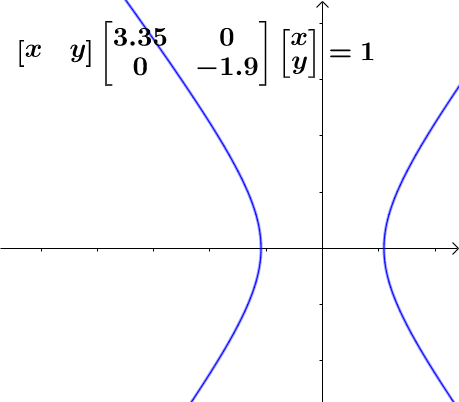
\includegraphics[width=.3\textwidth]{fig/UnderstandQuadraticForm_5.png}
\end{figure} 
双曲线和圆之间也是线性关系(准确的说是仿射的)。其实圆、椭圆、双曲线之间关系很紧密的,统称为圆锥曲线,都是圆锥体和平面的交线。一个平面在圆锥体上运动,可以得到圆、椭圆、双曲线,这也是它们之间具有线性关系的来源(平面的运动是线性的、或者是仿射的)。

\textbf{规范化}

再改变下矩阵:
\begin{figure}[H]
    \centering
    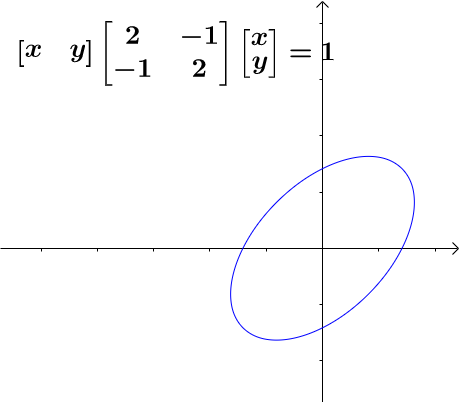
\includegraphics[width=.3\textwidth]{fig/UnderstandQuadraticForm_6.png}
\end{figure} 

这个椭圆看起来有点歪,不太好处理,我们来把它扶正,这就叫做\textbf{规范化}。如果我们对矩阵有更深刻的认识,那么要把它扶正很简单。

首先,矩阵代表了运动,包含:
\begin{itemize}
\setlength{\itemsep}{0pt}
\setlength{\parsep}{0pt}
\setlength{\parskip}{0pt}
    \item 旋转
    \item 拉伸
    \item 投影
\end{itemize}

对于方阵,因为没有维度的改变,所以就没有投影这个运动了,只有
\begin{itemize}
\setlength{\itemsep}{0pt}
\setlength{\parsep}{0pt}
\setlength{\parskip}{0pt}
    \item 旋转
    \item 拉伸
\end{itemize}

具体到上面的矩阵:
\begin{figure}[H]
    \centering
    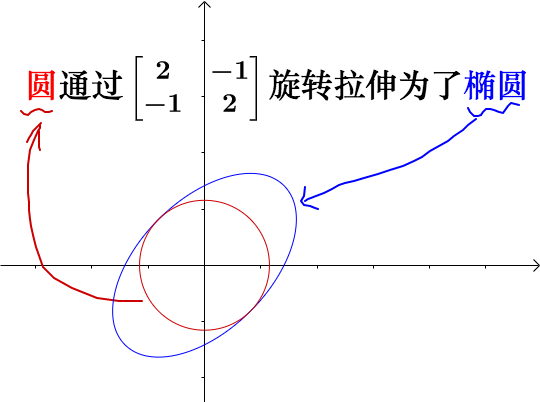
\includegraphics[width=.3\textwidth]{fig/UnderstandQuadraticForm_7.png}
\end{figure} 

我把这个矩阵进行特征值分解:
\begin{figure}[H]
    \centering
    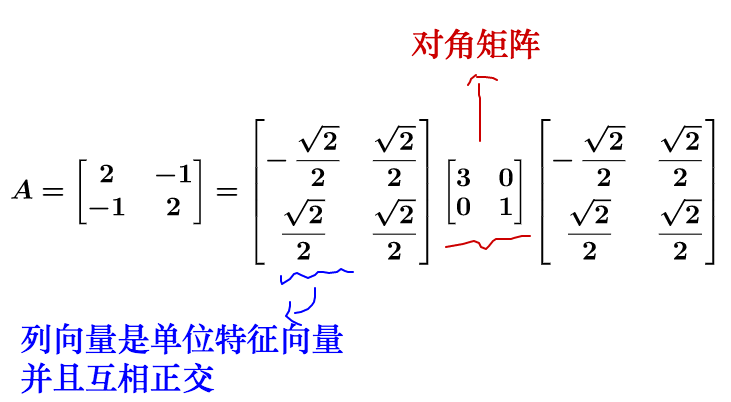
\includegraphics[width=.5\textwidth]{fig/UnderstandQuadraticForm_8.png}
\end{figure} 

对于二次型矩阵,都是对称矩阵,所以特征值分解总可以得到正交矩阵与对角矩阵。特征值分解实际上就是把运动分解了:
\begin{figure}[H]
    \centering
    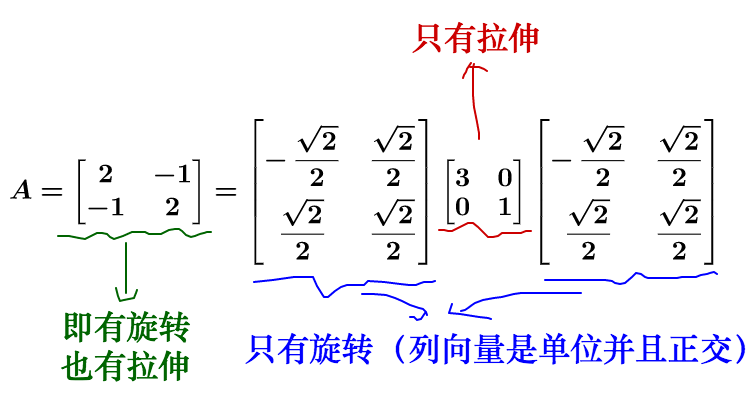
\includegraphics[width=.5\textwidth]{fig/UnderstandQuadraticForm_9.png}
\end{figure} 

那么我们只需要保留拉伸部分,就相当于把矩阵扶正(图中把各自图形的二次型矩阵标注出来了):
\begin{figure}[H]
    \centering
    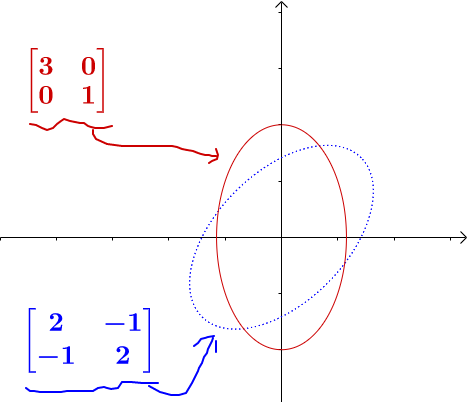
\includegraphics[width=.3\textwidth]{fig/UnderstandQuadraticForm_10.png}
\end{figure} 

所以,用二次型矩阵进行规范化是非常轻松的事情。

\textbf{正定}

正定是对二次函数有效的一个定义,对方程无效。对于二次型函数,$f(x)=x^TAx$:
\begin{itemize}
    \item $f(x)>0, x \ne 0, x \in \mathbb{R}$,则 $f$ 为正定二次型,$A$为正定矩阵
    \item $f(x) \ge 0, x \ne 0, x \in \mathbb{R}$,则 $f$ 为半正定二次型,$A$为半正定矩阵
    \item $f(x) < 0, x \ne 0, x \in \mathbb{R}$,则 $f$ 为负定二次型,$A$为负定矩阵
    \item $f(x) \le 0, x \ne 0, x \in \mathbb{R}$,则 $f$ 为半负定二次型,$A$为半负定矩阵
    \item 以上皆不是,就叫做不定
\end{itemize}

从图像上看,这是正定:
\begin{figure}[H]
    \centering
    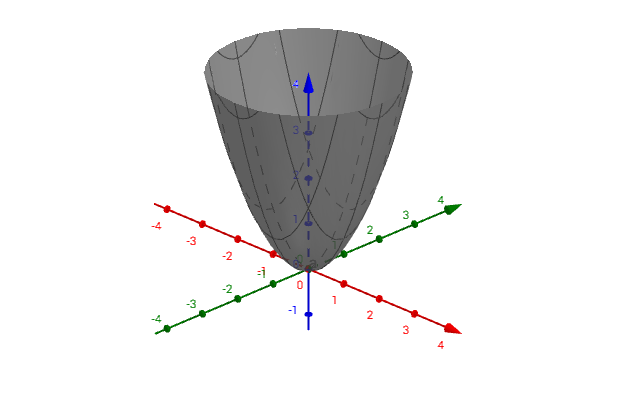
\includegraphics[width=.5\textwidth]{fig/UnderstandQuadraticForm_11.png}
\end{figure} 

半正定:
\begin{figure}[H]
    \centering
    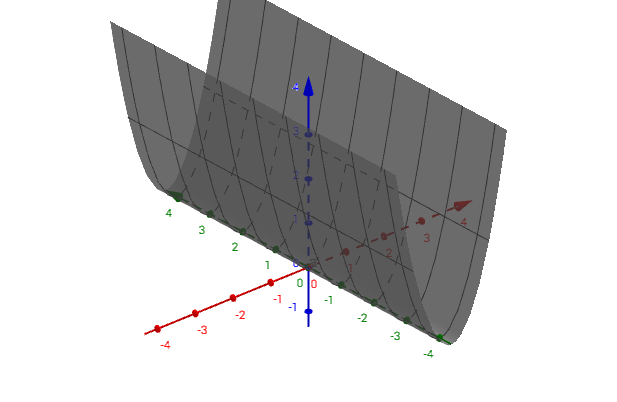
\includegraphics[width=.5\textwidth]{fig/UnderstandQuadraticForm_12.png}
\end{figure} 

不定:
\begin{figure}[H]
    \centering
    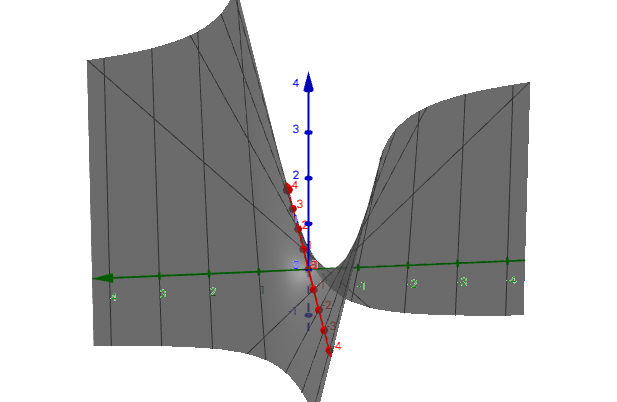
\includegraphics[width=.5\textwidth]{fig/UnderstandQuadraticForm_13.png}
\end{figure} 

既然二次型用矩阵来表示了,那么我们能否通过矩阵来判断是否正定呢?\textbf{如果矩阵的特征值都大于0,则为正定矩阵。}

\section{理解矩阵特征值和特征向量\cite{How_To_Understand_Eigen_Value_Vector}}
假设我们有一个$n$阶的矩阵$A$以及一个实数$\lambda$,使得我们可以找到一个非零向量$\vec{x}$,满足:
$$
A\vec{x} = \lambda\vec{x}
$$

如果能够找到的话,我们就称$\lambda$是矩阵$A$的特征值,非零向量$\vec{x}$是矩阵$A$的特征向量。

先给一个简短的回答,如果把矩阵看作是运动,对于运动而言,最重要的当然就是运动的速度和方向,那么(我后面会说明一下限制条件):
\begin{itemize}
    \item 特征值就是运动的速度
    \item 特征向量就是运动的方向
\end{itemize}

既然运动最重要的两方面都被描述了,特征值、特征向量自然可以称为运动(即矩阵)的特征。

注意,由于矩阵是数学概念,非常抽象,所以上面所谓的运动、运动的速度、运动的方向都是广义的,在现实不同的应用中有不同的指代。

\subsection{几何意义}
给定标准基$\vec{i},\vec{j}$和向量$\vec{v}$:
\begin{figure}[H]
    \centering
    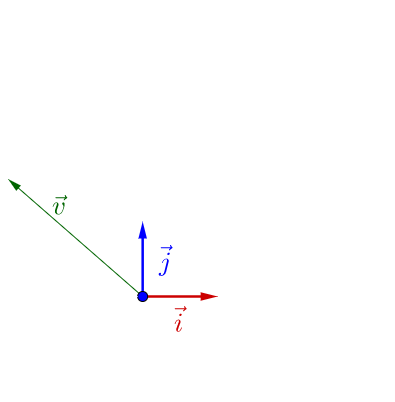
\includegraphics[width=.3\textwidth]{fig/UnderstandEigenValueVector_1.png}
\end{figure} 

随便左乘一个矩阵$A$,图像看上去没有什么特殊的:
\begin{figure}[H]
    \centering
    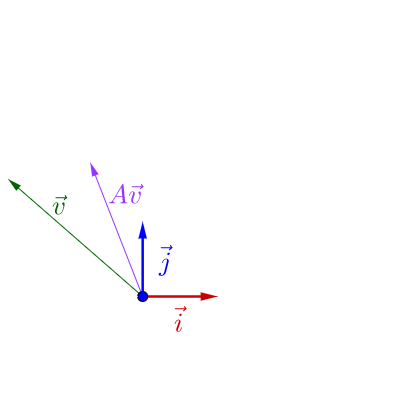
\includegraphics[width=.3\textwidth]{fig/UnderstandEigenValueVector_2.png}
\end{figure} 

但是调整下$\vec{v_{}}$的方向,图像看上去就有点特殊了:
\begin{figure}[H]
    \centering
    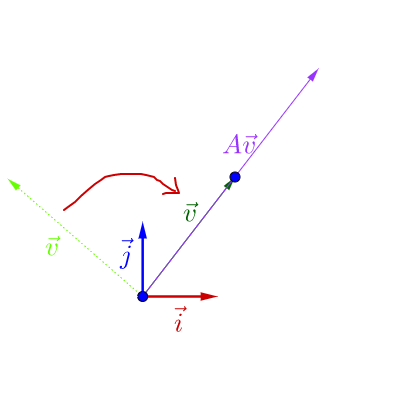
\includegraphics[width=.3\textwidth]{fig/UnderstandEigenValueVector_3.png}
\end{figure} 

可以观察到,调整后的$\vec{v_{}}$和$A\vec{v_{}}$在同一根直线上,只是$A\vec{v_{}}$的长度相对$\vec{v_{}}$的长度变长了。

此时,我们就称\textbf{$\vec{v_{}}$是$A$的特征向量,而$A\vec{v_{}}$的长度是$\vec{v_{}}$的长度的$\lambda$倍,$\lambda$就是特征值}。

从而,特征值与特征向量的定义式就是这样的:

\begin{figure}[H]
    \centering
    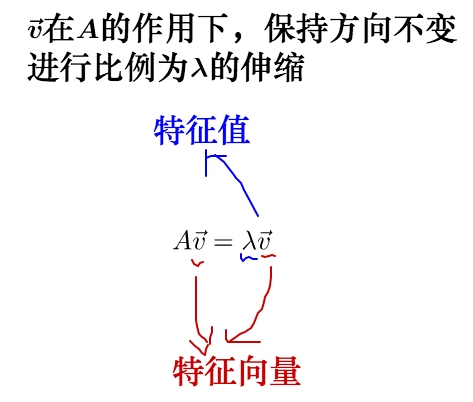
\includegraphics[width=.5\textwidth]{fig/UnderstandEigenValueVector_4.png}
\end{figure} 

其实之前的A不止一个特征向量,还有另一个特征向量:
\begin{figure}[H]
    \centering
    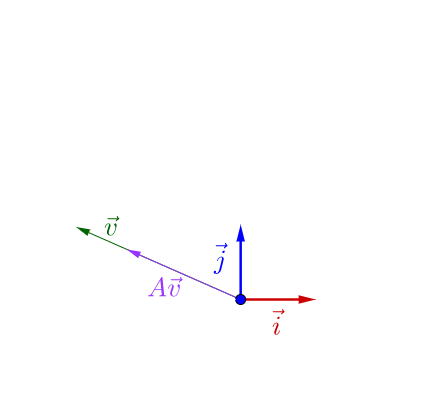
\includegraphics[width=.3\textwidth]{fig/UnderstandEigenValueVector_5.png}
\end{figure} 

容易从$A\vec{v_{}}$相对于$\vec{v_{}}$是变长了还是缩短看出,这两个特征向量对应的特征$\lambda$值,一个大于1,一个小于1。

从特征向量和特征值的定义式还可以看出,特征向量所在直线上的向量都是特征向量:
\begin{figure}[H]
    \centering
    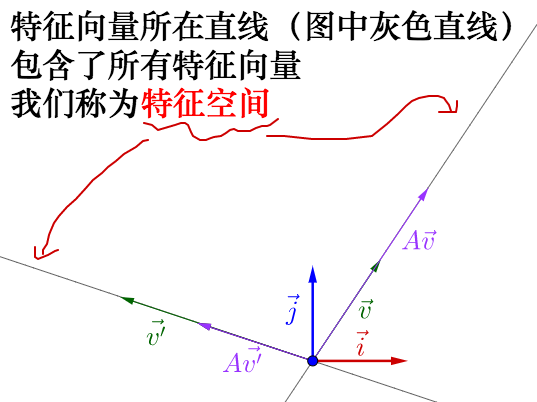
\includegraphics[width=.3\textwidth]{fig/UnderstandEigenValueVector_6.png}
\end{figure} 

\subsection{从公式进一步理解特征值\cite{Eigen_Value_And_Sigular_Value}}
回到特征值和特征向量的定义:$$
A\vec{v} = \lambda\vec{v}
$$

可以看出来该公式有如下特点:
\begin{itemize}
    \item $A$ 为(作用)方阵;
    \item $v$是$A$的特征向量;
    \item $\lambda$ 是 $A$ 的特征值,为纯量,就是一个数,可以表示为对角阵。
\end{itemize}

让我们根据这个式子展开想象:

矩阵的乘法都是线性变换,式子想说明,特征向量在$A$ 的作用下进行线性变换,效果是特征向量的 $\lambda$ 倍伸缩。注意:

\begin{itemize}
    \item 并不是所有向$A$都能被伸缩,只有$\vec{v}$ 中的向量(特征向量)能被其伸缩;
    \item 伸缩的尺度 $\lambda$ 体现 $A$ 的变换能力。
\end{itemize}

这样的话,\textbf{如果我们知道了一个方阵的特征值和特征向量,就知道了这个方阵的线性变换能力}。

放到应用场景中就是,我们通过特征值就能掌握当前数据在对应方向上的变换能力。所以某些场景中,我们选取较大的特征值们来代表原数据的变换能力,例如:PCA分析、数据压缩。

\subsection{特征值、特征向量与运动的关系}
\subsubsection{矩阵的混合}
一般来说,矩阵我们可以看作某种运动,而二维向量可以看作平面上的一个点(或者说一个箭头)。对于点我们是可以观察的,但是运动我们是不能直接观察的。要观察矩阵所代表的运动,需要把它附加到向量上才观察的出来。

单独做一次矩阵的左乘(运动):
\begin{figure}[H]
    \centering
    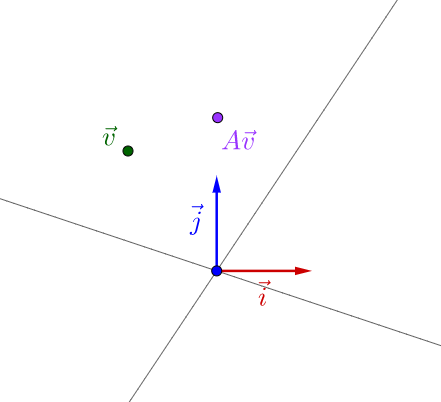
\includegraphics[width=.3\textwidth]{fig/UnderstandEigenValueVector_7.png}
\end{figure} 

似乎还看不出什么。但是如果我反复运用矩阵乘法的话:
\begin{figure}[H]
    \centering
    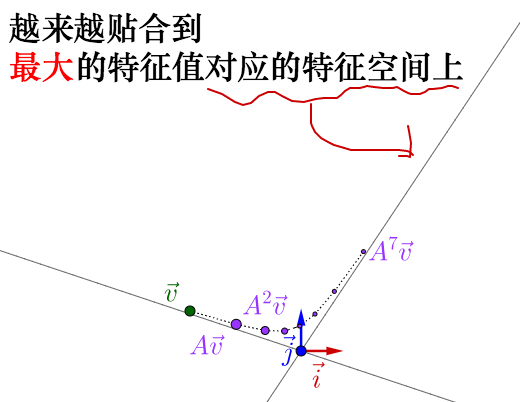
\includegraphics[width=.5\textwidth]{fig/UnderstandEigenValueVector_8.png}
\end{figure} 

也就是说,反复运用矩阵乘法,矩阵所代表的运动的最明显的特征,即速度最大的方向,就由最大特征值对应的特征向量展现了出来。

但是,上面的推论有一个重要的条件:特征向量正交,这样变换后才能保证变换最大的方向在基方向。如果特征向量不正交就有可能不是变化最大的方向。所以我们在实际应用中,都要去找正交基。但是特征向量很可能不是正交的,那么我们就需要奇异值分解了。

\subsection{特征值分解}
我们知道,对于矩阵$A$可以对角化的话,可以通过相似矩阵进行下面这样的特征值分解:
$$
A = P\Lambda P^{-1}
$$

其中$\Lambda$为对角阵,$P$的列向量是单位化的特征向量。

\begin{framed}  
%\verb|\documentstyle[ifthen,12pt,titlepage]{article}|
\small{
证明方法:

给定矩阵$A_{n*n}$的$n$个线性无关的特征向量,按列组成方阵,即:
$$
S: [\vec{x_1}, \vec{x_2}, \cdots, \vec{x_n}]
$$

那么有:
\begin{align*}
    AS &= A[\vec{x_1}, \vec{x_2}, \cdots, \vec{x_n}] \\
    &= [\lambda_1\vec{x_1}, \lambda_2\vec{x_2}, \cdots, \lambda_n\vec{x_n}] \\
    &= [\vec{x_1}, \vec{x_2}, \cdots, \vec{x_n}] \Lambda \\
    &= S\Lambda
\end{align*}

其中$\Lambda$为特征值组成的对角矩阵,因为假设组成特征向量矩阵 $S$ 的 $n$ 个特征向量线性无关,所以 $S$ 可逆,从上式中就可以推导出对角化以及特征值分解的公式:
\begin{align*}
    &S^{-1}AS = \lambda \\
    &A = S^{-1}\lambda S
\end{align*}
}
\end{framed}

说的有点抽象,我们拿个具体的例子来讲:
$$
A= \begin{bmatrix}
2&-1\\-1&2
\end{bmatrix}
$$

按照后文的特征值的计算方法计算后可知:
\begin{align*}
    \lambda_1 = 3 &\Rightarrow \vec{x_1} = \begin{bmatrix}
    -\frac{\sqrt{2}}{2} \\ \frac{\sqrt{2}}{2}
    \end{bmatrix} \\
    \lambda_2 = 1 &\Rightarrow \vec{x_2} = \begin{bmatrix}
    \frac{\sqrt{2}}{2} \\ \frac{\sqrt{2}}{2}
    \end{bmatrix}
\end{align*}

所以有:
\begin{figure}[H]
    \centering
    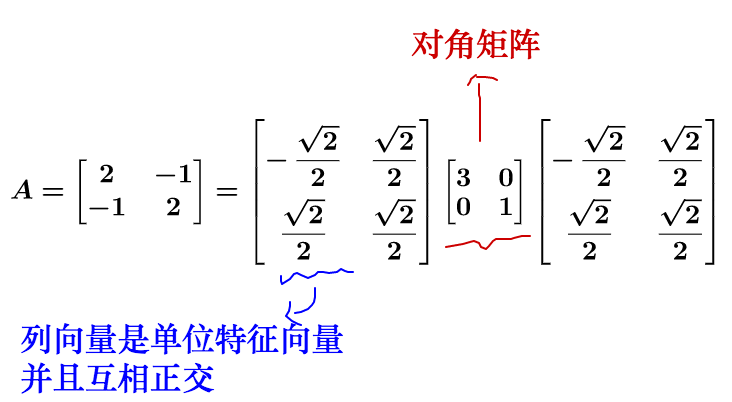
\includegraphics[width=.5\textwidth]{fig/UnderstandEigenValueVector_9.png}
\end{figure} 

对于方阵而言,矩阵不会进行维度的升降,所以矩阵代表的运动实际上只有两种:旋转和拉伸,所以最后的运动结果就是这两种的合成。

我们再回头看下刚才的特征值分解,实际上把运动给分解开了:
\begin{figure}[H]
    \centering
    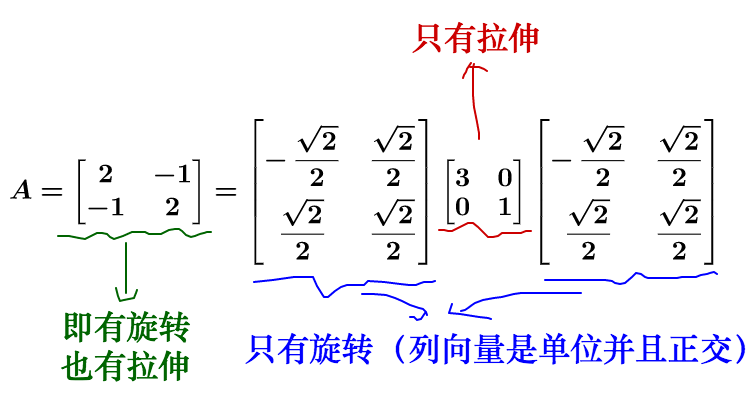
\includegraphics[width=.5\textwidth]{fig/UnderstandEigenValueVector_10.png}
\end{figure} 

\subsubsection{特征值分解的条件}
矩阵可以被特征值分解的条件为:
\begin{enumerate}
    \item \textbf{矩阵是方阵。(SVD分解无此要求);}
    \item 方阵$A_{n\times n}$可以做特征值分解的充要条件是其有 $n$ 个线性无关的特征向量。
\end{enumerate}

\subsection{特征值、特征向量的应用}
\textbf{特征值越大,说明矩阵在对应的特征向量上的方差越大,功率越大,信息量越多。}

应用到最优化中,意思就是对于R的二次型,自变量在这个方向上变化的时候,对函数值的影响最大,也就是该方向上的方向导数最大。

应用到数据挖掘中,意思就是最大特征值对应的特征向量方向上包含最多的信息量,如果某几个特征值很小,说明这几个方向信息量很小,可以用来降维,也就是删除小特征值对应方向的数据,只保留大特征值方向对应的数据,这样做以后数据量减小,但有用信息量变化不大。

\subsubsection{控制系统}
当 $\lambda = 1时$,系统最终会趋于稳定。
\begin{figure}[H]
    \centering
    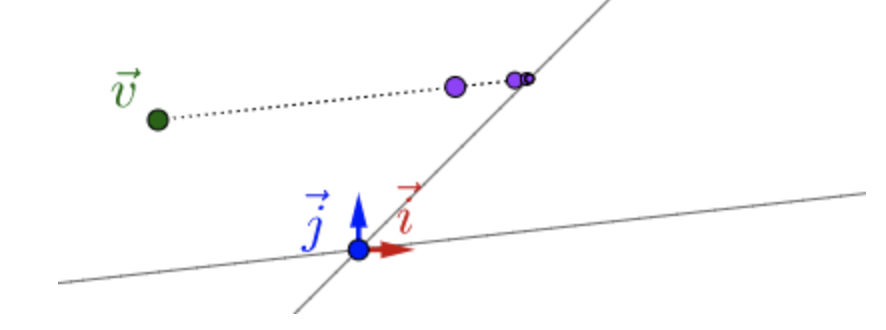
\includegraphics[width=.5\textwidth]{fig/UnderstandEigenValueVector_11.png}
\end{figure} 

\subsubsection{图片压缩}
比如说,有下面这么一副$512\times512$的图片(方阵才有特征值,所以找了张正方形的图):
\begin{figure}[H]
    \centering
    \includegraphics[width=.3\textwidth]{fig/UnderstandEigenValueVector_12.jpg}
\end{figure} 

这个图片可以放到一个矩阵里面去,就是把每个像素的颜色值填入到一个$512\times512$的矩阵$A$中。

根据之前描述的有:
$$
A = P\Lambda P^{-1}
$$
其中,$\Lambda$是对角阵,对角线上是从大到小排列的特征值。

我们在[公式]中只保留前面50个的特征值(也就是最大的50个,其实也只占了所有特征值的百分之十),其它的都填0,重新计算矩阵后,恢复为下面这样的图像:
\begin{figure}[H]
    \centering
    \includegraphics[width=.3\textwidth]{fig/UnderstandEigenValueVector_13.jpg}
\end{figure} 

效果还可以,其实一两百个特征值之和可能就占了所有特征值和的百分之九十了,其他的特征值都可以丢弃了。

\subsubsection{二次型最优化问题}
二次型$y = x^TRx$,其中$R$是已知的二阶矩阵,$y = [1, 0.5;0.5, 1]$,$x$是二维列向量,$x=[x_1; x_2]$,求 $y$ 的最小值。

求解很简单,讲一下这个问题与特征值的关系。对$R$特征分解,特征向量是$[-0.7071;0.7071]$和$[0.7071;0.7071]$,对应的特征值分别是0.5和1.5。
然后把$y$的等高线图画一下:
\begin{figure}[H]
    \centering
    \includegraphics[width=.3\textwidth]{fig/UnderstandEigenValueVector_14.jpg}
\end{figure} 

从图中看,函数值变化最快的方向,也就是曲面最陡峭的方向,归一化以后是[0.7071;0.7071],嗯哼,这恰好是矩阵R的一个特征值,而且它对应的特征向量是最大的。因为这个问题是二阶的,只有两个特征向量,所以另一个特征向量方向就是曲面最平滑的方向。这一点在分析最优化算法收敛性能的时候需要用到。二阶问题比较直观,当R阶数升高时,也是一样的道理。

\subsection{特征值的计算方法}
我们对原式来进行一个很简单的变形:
\begin{align*}
    A\vec{x} &= \lambda\vec{x} \\
    (A - \lambda I)\vec{x} &= 0
\end{align*}
这里的$I$表示单位矩阵,如果把它展开的话,可以得到一个$n$元的齐次线性方程组。这个我们已经很熟悉了,这个齐次线性方程组要存在非零解,那么需要系数行列式
$$
|A - \lambda I| = 0
$$

(原文疑似有误,这里已修正,待验证)

我们将这个行列式展开:
$$
\begin{vmatrix}
a_{11} - \lambda & a_{12} & \cdots & a_{1n} \\
a_{21} & a_{22} - \lambda & \cdots & a_{2n} \\
\vdots & \vdots & & \vdots \\
a_{n1} & a_{n2} & \cdots & a_{nm} - \lambda
\end{vmatrix}
$$

这是一个以$\lambda$为未知数的一元$n$次方程组,$n$次方程组在复数集内一共有$n$个解。我们观察上式,可以发现$\lambda$只出现在正对角线上,显然,$A$的特征值就是方程组的解。因为$n$次方程组有$n$个复数集内的解,所以矩阵$A$在复数集内有$n$个特征值。

我们举个例子,尝试一下:
$$
A = 
\begin{bmatrix}
a_{11} - \lambda & a_{12} \\
a_{21} & a_{22} - \lambda
\end{bmatrix}
$$

那么 $f(\lambda) = (a_{11}-\lambda)(a_{22}-\lambda) - a_{12}a_{21} = \lambda^2 - (a_{11}+a{22})\lambda + |A|$,我们套入求根公式可以得出使得$f(\lambda)=0$的两个根 $\lambda_1, \lambda_2$,有:
\begin{align*}
    \lambda_1 + \lambda_2 &= a_{11} + a_{22} \\
    \lambda_1\lambda_2 &= |A|
\end{align*}

这个结论可以推广到所有的$n$都可以成立,也就是说对于一个$n$阶的方阵$A$,都可以得到:
\begin{align*}
    \lambda_1 + \lambda_2 + \cdots + \lambda_n &= a_{11} + a_{22} + \cdots + a_{nn} \\
    \lambda_1\lambda_2\cdots\lambda_n &= |A|
\end{align*}

\begin{framed}  
%\verb|\documentstyle[ifthen,12pt,titlepage]{article}|
\small{
参考\cite{The_Matrix_Cookbook},对于$2\times 2$的矩阵$A = [A_{11}, A_{12};A_{21}, A_{22}]$,有:

行列式和迹:
$$
det(A) = A_{11}A_{22} - A_{12}A_{21}
$$
$$
Tr(A) = Tr(A_{11}) + Tr(A_{11}) 
$$

特征值:
$$
\lambda^2 - \lambda \cdot Tr(A) + det(A) = 0    
$$
$$
\lambda_1 = \frac{Tr(A)+\sqrt{Tr(A)^2 - 4det(A)}}{2} \quad
\lambda_2 = \frac{Tr(A)-\sqrt{Tr(A)^2 - 4det(A)}}{2}
$$
$$
\lambda_1 + \lambda_2 = Tr(A) \quad \lambda_1\lambda_2 = det(A)
$$

特征向量:
$$
v_1 \propto \begin{bmatrix}
A_{12} \\ \lambda_1 - A_{11}
\end{bmatrix}
\quad
v_2 \propto \begin{bmatrix}
A_{12} \\ \lambda_2 - A_{11}
\end{bmatrix}
$$

逆:
$$
A^{-1} = \frac{1}{det(A)}\begin{bmatrix}
A_{22} & -A_{12} \\
A_{21} & A_{11}
\end{bmatrix}
$$
}
\end{framed}

\subsection{旋转矩阵只有复数特征值}
可以想一下,对于旋转矩阵,除了零向量。没有其他向量可以在平面上旋转而不改变方向的,所以旋转矩阵对应的矩阵没有实数特征值和实数特征向量,但是有复数特征特征值和特征向量。而且特征值和特征 向量是成对出现的。将特征值写成指数形式,它的幅值代表伸长或者缩小的程度,相角代表$Ax$ 和 $x$ 之间的夹角。

例如,当 $\theta = 30^\circ$ 时,对应的旋转矩阵为:
$$
T = \begin{bmatrix}
\frac{\sqrt{3}}{2} & -\frac{1}{2} \\
\frac{1}{2} & \frac{\sqrt{3}}{2}
\end{bmatrix}
$$

求解$|T-\lambda I| = 0$,有:
$$
\lambda_{1,2} = \frac{\sqrt{3}}{2} \pm \frac{1}{2}i
$$

更通用的形式:
$$
T =  \begin{bmatrix}
a & -b \\ b & a
\end{bmatrix}
$$

求解$|T-\lambda I| = 0$,有:
$$
\lambda_{1,2} = a \pm \sqrt{-b^2} = a \pm bi
$$

\subsection{常见变换对应的特征值和特征向量}
\begin{figure}[H]
    \centering
    \includegraphics[width=1.0\textwidth]{fig/EigenValueVectorsCommon.jpg}
    \caption*{最后一列貌似有问题,见下方证明}
\end{figure} 
\begin{framed}  
%\verb|\documentstyle[ifthen,12pt,titlepage]{article}|
\small{
证明:
\begin{align*}
M_1 &= [k,0;0,k] \rightarrow (k-\lambda)^2 = 0 \rightarrow \lambda_1 = \lambda_2 = k \\
M_2 &= [k_1,0;0,k_2] \rightarrow (k_1 - \lambda)(k_2 - \lambda) = 0 \rightarrow \lambda_1 = k_1, \lambda_2 = k_2 \\
M_3 &= [c, -s; s, c], c = \cos\theta, s = \sin\theta \rightarrow  \lambda^2 - 2c\lambda + 1 = 0\rightarrow \lambda_1 = c + s\mathbf{i}, \lambda_2 = c - s\mathbf{i} \\
M_4 &= [1,k;0,1],  \rightarrow  (\lambda-1)^2 = 0 \rightarrow \lambda_1 = \lambda_2 = 1 \\
M_5 &= [c, s; s, c], c = \cos\theta, s = \sin\theta \rightarrow  \lambda^2 - 2c\lambda + c^2 - s^2 = 0\rightarrow \lambda_1 = c + s, \lambda_2 = c - s \\
\end{align*}
}
\end{framed}

\subsection{特征值的性质\cite{Eigen_Value_And_Eigen_Vector_Zhihu}}
\subsubsection{特征值和迹、行列式的关系}
$$
\lambda_1 + \lambda_2 + \cdots + \lambda_n = tr(A)
$$
$$
\lambda_1 \cdot \lambda_2 \cdot \cdots \cdot \lambda_n = det(A)
$$

\subsubsection{特征值的幂}
已知:
$$
A\mathbf{x} = \lambda\mathbf{x}
$$

有:
$$
A^2\mathbf{x} = A(A\mathbf{x}) = A(\lambda\mathbf{x}) = \lambda(A\mathbf{x}) = \lambda^2\mathbf{x}
$$

也就是 $A^2$ 特征值为 $\lambda^2$ ,特征向量跟$A$相同,还可以继续推出:
$$
A^k\mathbf{x} = \lambda^k\mathbf{x}
$$
$$
A^{-1}\mathbf{x} = \frac{1}{\lambda}\mathbf{x}
$$

同时这里我们可能会想要注意 $\lambda \ne 0$ ,但实际上如果$\lambda = 0$,那就是 $A\mathbf{x} = 0$ , $A$不可逆。

还有:
$$
e^{At}\mathbf{x} = e^{\lambda t}\mathbf{x}
$$

这个式子的推导可以用泰勒展开:
$$
e^x = \sum_{n=0}^{\infty}\frac{x^n}{n!} = 1 + x + \frac{x^2}{2!} + \frac{x^3}{3!} + \cdots
$$

实际上最早特征值和特征向量就是为了解决微分方程出现的。

还有:如果$n \times n$ 矩阵有 $n$ 个特征向量,我们当然就可以用它来做一组基,可以把空间中任何向量写成:
$$
\mathbf{v} = c_1\mathbf{x} + \cdots + c_n\mathbf{x}
$$
\begin{align*}
A^k\mathbf{v} &= A^kc_1\mathbf{x_1} + \cdots + A^kc_n\mathbf{x_n} \\
    &= c_1A^k\mathbf{x_1} + \cdots + c_nA^k\mathbf{x_n} \\
   &= c_1\lambda_1^k\mathbf{x_1} + \cdots + c_n\lambda_1^k\mathbf{x_n} \\
\end{align*}


\subsection{矩阵的特征值和”谱“\cite{Fantastic_Matrix_1}}
矩阵的特征值有时会被称为谱,这和特征值的物理意义有关。如果你学过线性系统理论或者振动分析类的课程,就会知道,一阶线性微分方程组对应的矩阵的特征值,就是系统的固有频率。我们知道,凡是叫谱的东西,都是可以分解的,比如光谱。那么这个矩阵可不可以 分解呢?答案是肯定的:我们可以将一个具有良好性能的矩阵分解成多个作用的叠加。

在数学中有一个谱定律(Spectral theorem),也叫谱分解或者特征值分解。它的核心内 容如下:一个矩阵 $A$ 可表示为如下线性组合
$$
A = \lambda_1 P_1 + \lambda_2 P_2 + \lambda_3 P_3 +  \cdots
$$

其中,$P_1, P_2, P_3, \cdots, P_n $称为 $A$ 的谱族,$\lambda_1, \lambda_2, \lambda_3, \cdots, \lambda_n$等表示特征值。

这里做了两个假设:1) 矩阵 $A$ 是可以对角化的;2)所有特征值都是不同的(这个不是必须的,只是为了结果比较清晰)。

对于可对角化的矩阵 $A$ 我们可以将它表示成这样:
$$
A = P
\begin{bmatrix}
\lambda_1 & & & \\
& \lambda_2 & & \\
& & \ddots & \\
& & & \lambda_n 
\end{bmatrix}
P^{-1}
$$

这里将 $P$ 拆成列向量, $P^{-1}$ 拆成行向量:$P = [p_1, p_2, \cdots, p_n], P^{-1} = [q_1, q_2, \cdots, q_n]^T$,于是可以得到矩阵:
$$
P_1 = p_1q_1, P_2 = p_2q_2, \cdots, P_n = p_nq_n, 
$$

如果特征值相同,只要矩阵 $A$ 可对角化,上面的分解也是可以进行的。把相同特征值的 块合并在一起就可以,从它的应用角度来说这样处理是合理的。

从这里我们可以看出,\textbf{一个变换(矩阵)可由它的所有特征值和谱族完全表示。特征值 和谱族的乘积就代表了它对矩阵 $A$ 的贡献率}——说的通俗一点就是能量(power)或者权重 (weight)。这样,能量多的、权重大的部分当然重要,问题的主要矛盾就凸显出来了!当 然,也可以这样理解:把特征值看成坐标,谱族看成基。于是,一组基+一组坐标就表示了一个对象——矩阵 $A$。

\section{理解迹\cite{How_To_Understand_Trace}}
线性代数中,把方阵的对角线之和称为“迹”,即对于给定的矩阵:
$$
A = \begin{pmatrix}
a_{11} & a_{12} & \cdots & a_{1n} \\
a_{21} & a_{22} & \cdots & a_{2n} \\
\vdots & \vdots & & \vdots \\
a_{n1} & a_{n2} & \cdots & a_{nn} \\
\end{pmatrix}
$$
$$
Tr(A) = \sum_i^na_{ii}
$$

“迹”就是线性变换藏在矩阵中痕迹。

\subsection{迹的性质}
已知$A,B$是两个$n\times n$的矩阵,$k$是一个常数,则:
\begin{itemize}
\setlength{\itemsep}{0pt}
\setlength{\parsep}{0pt}
\setlength{\parskip}{0pt}
    \item $tr(kA) = k\cdot tr(A)$
    \item $tr(A+B) = tr(A) + tr(B)$
    \item $tr(AB) = tr(BA)$
    \item 
\end{itemize}

\section{再论相似矩阵}
\subsection{相似矩阵的“迹”、行列式、特征值的关系}
给定矩阵$A$、$B$,已知$A,B$互为相似矩阵,即$B = P^{-1}AP$,那么:

\subsubsection{迹}
相似矩阵的“迹”都相等。证明如下:
\begin{align*}
    B &= P^{-1}AP \Rightarrow \\
    tr(B) &= tr(P^{-1}AP) \\
          &= tr(P^{-1}(AP)) \\
          &= tr((AP)P^{-1}) \\
          &= tr(A) \\   
\end{align*}

\subsubsection{行列式}
因为$A,B$代表同一个线性变换,而根据行列式的意义,行列式代表的是线性变换的伸缩比例。既然是比例,那么也和坐标无关,即:
$$
det(A) = det(B) = 1
$$

所以行列式是一个相似不变量。

\subsubsection{特征值}
根据特征值分解的定义,特征值矩阵$\Lambda$:
$$
\Lambda = Q^{-1}AQ
$$

这里用$Q$是为了和之前的$P$进行区别。可见,$\Lambda$和$A$,$B$也是相似矩阵。所以:

对$A,B$求特征值矩阵都得到的是同一个$\Lambda$(特征向量有所不同,因为在不同的基下)

\subsubsection{结论}
更一般的,可以得到这两个相似不变量和特征值的关系分别为:
\begin{itemize}
    \item 迹 = $\lambda_1 + \lambda_2 + \cdots$
    \item 行列式 = $\lambda_1\cdot\lambda_1\cdots$
\end{itemize}


\section{理解奇异值\cite{How_To_Understand_Singular_Value}}
奇异值与特征值相对应。特征值固然方便使用,但其对原矩阵为\textbf{方阵}的限制为实际情况下所难得的。自然,我们就需要一种更一般化的特征提取方式,这里的特征我们叫奇异值(singular value),而这种方式正是奇异值分解(singular-value decomposition (SVD))。所以,该分解和结果的意义与特征值类似,但拓展了适用范围\cite{Eigen_Value_And_Sigular_Value}。

\subsection{定义}
$$
M = U\Sigma V^* \Rightarrow 
\begin{cases}
M: m\times n\text{矩阵} \\
N: m\times m\text{酉矩阵,} U\text{的列是}M\text{的正交}\textbf{输出}\text{基向量}\\
\Sigma: m\times n\text{的对角阵,对角元素非负(奇异值);其余元素均为 0} \\
V^*: n\times n\text{酉矩阵,是}V \text{的转置,}V\text{的列是}M\text{的正交}\textbf{输入}\text{基向量}
\end{cases}
$$

注: $N$和 $V$都是酉矩阵(unitary matrix),即满足:
$$
U^TU = I, V^TV = I
$$

需要注意的是,\textbf{奇异值分解结果并不唯一。}

\subsubsection{与特征值分解的关系\cite{Eigen_Value_And_Sigular_Value_Relation}}
首先,矩阵可以认为是一种线性变换,而且这种线性变换的作用效果与基的选择有关。以$Ax = b$为例,$x$是$m$维向量,$b$是$n$维向量,$m,n$可以相等也可以不相等,表示矩阵可以将一个向量线性变换到另一个向量,这样一个线性变换的作用可以包含\textbf{旋转、缩放和投影}三种类型的效应。

奇异值分解正是\textbf{对线性变换这三种效应的一个析构}。给定奇异值分解$A = \mu\Sigma\sigma^T$,$\mu,\sigma$是\textbf{两组正交单位向量},$\Sigma$是对角阵,表示奇异值;它表示我们找到了$\mu,\sigma$这样两组基,$A$矩阵的作用是将一个向量从$\sigma$这组正交基向量的空间\textbf{旋转}到$\mu$这组正交基向量空间,并对每个方向进行了一定的\textbf{缩放},缩放因子就是各个\textbf{奇异值}。如果$\sigma$维度比$\mu$大,则表示还进行了投影。可以说奇异值分解将一个矩阵原本混合在一起的三种作用效果,分解出来了。

而特征值分解其实是\textbf{对旋转和缩放两种效应的归并}(有投影效应的矩阵不是方阵,没有特征值)。特征值,特征向量由$Ax=\lambda x$得到,它表示如果一个向量$v$处于$A$的特征向量方向,那么$Av$对$v$的线性变换作用只是一个\textbf{缩放}。也就是说,求特征向量和特征值的过程,我们找到了这样一组基,在这组基下,矩阵的作用效果仅仅是存粹的\textbf{缩放}。对于实对称矩阵,特征向量正交,我们可以将特征向量式子写成$A=x\lambda x^T$,这样就和奇异值分解类似了,就是$A$矩阵将一个向量从$x$这组基的空间旋转到$x$这组基的空间,并在每个方向进行了缩放,由于前后都是$x$,就是没有旋转或者理解为旋转了0度。

总结一下,特征值分解和奇异值分解都是\textbf{给一个矩阵(线性变换)找一组特殊的基}:
\begin{itemize}
    \item 特征值分解找到了特征向量这组基,在这组基下该线性变换只有缩放效果。
    
    \item 奇异值分解则是找到另一组基,这组基下线性变换的旋转、缩放、投影三种功能独立地展示出来了
\end{itemize}

特征值分解其实是一种找特殊角度,让旋转效果不显露出来,所以并不是所有矩阵都能找到这样巧妙的角度。仅有缩放效果,表示、计算的时候都更方便,但是这样的基很多时候不再正交了,又限制了一些应用。

\subsection{通俗理解奇异值分解}
给定一个变换矩阵 $A = [1, -2;1, 2]$,通过一个单位圆来观察:
\begin{figure}[H]
    \centering
    \includegraphics[width=.3\textwidth]{fig/UnderstandSingularValue_1.png}
\end{figure} 

把这个单位圆的每一点都通过$A$进行变换,得到一个椭圆(我把单位圆保留下来了,作为一个比较):
\begin{figure}[H]
    \centering
    \includegraphics[width=.3\textwidth]{fig/UnderstandSingularValue_2.png}
\end{figure} 

对 $A$ 进行奇异值分解:
\begin{align*}
    A &= \begin{bmatrix}1&-2\\1&2\end{bmatrix} \\
    &= \begin{bmatrix}-0.707&-0.707\\0.707&-0.707\end{bmatrix} 
    \begin{bmatrix}2.828&0\\0&1.414\end{bmatrix}
    \begin{bmatrix}0&-1\\1&0\end{bmatrix}
\end{align*}

实际上,将$A$分为了两个“分力”:
$$
 A  = \begin{bmatrix}-0.707&-0.707\\0.707&-0.707\end{bmatrix} 
    \begin{bmatrix}2.828&0\\0&0\end{bmatrix}
    \begin{bmatrix}0&-1\\1&0\end{bmatrix} + 
    \begin{bmatrix}-0.707&-0.707\\0.707&-0.707\end{bmatrix} 
    \begin{bmatrix}0&0\\0&1.414\end{bmatrix}
    \begin{bmatrix}0&-1\\1&0\end{bmatrix}
$$

我们来看看第一个“分力”,$\begin{bmatrix}-0.707&-0.707\\0.707&-0.707\end{bmatrix}\begin{bmatrix}2.828&0\\0&0\end{bmatrix}\begin{bmatrix}0&-1\\1&0\end{bmatrix}=\begin{bmatrix}0&-2\\0&2\end{bmatrix}$,作用在单位圆这个“橡皮筋”上的效果:
\begin{figure}[H]
    \centering
    \includegraphics[width=.3\textwidth]{fig/UnderstandSingularValue_3.png}
\end{figure} 

可怜的“橡皮筋”被拉成了一根线段。

我们来看看第二个“分力”,$\begin{bmatrix}-0.707&-0.707\\0.707&-0.707\end{bmatrix}\begin{bmatrix}0&0\\0&1.414\end{bmatrix}\begin{bmatrix}0&-1\\1&0\end{bmatrix}=\begin{bmatrix}1&0\\1&0\end{bmatrix}$,作用在单位圆这个“橡皮筋”上的效果:
\begin{figure}[H]
    \centering
    \includegraphics[width=.3\textwidth]{fig/UnderstandSingularValue_4.png}
\end{figure} 

可怜的“橡皮筋”被拉成了另外一根线段。

这两个“分力”一起作用的时候,可以想象(画面自行脑补),单位圆这个“橡皮筋”被拉成了椭圆:
\begin{figure}[H]
    \centering
    \includegraphics[width=.3\textwidth]{fig/UnderstandSingularValue_5.png}
\end{figure} 

\subsubsection{奇异值的物理解释}
同上文,奇异值分解实际上把矩阵的变换分为了三部分:
\begin{itemize}
\setlength{\itemsep}{0pt}
\setlength{\parsep}{0pt}
\setlength{\parskip}{0pt}
    \item 旋转
    \item 拉伸
    \item 投影
\end{itemize}

举例子(方阵没有投影,不过不影响这里思考):
\begin{figure}[H]
    \centering
    \includegraphics[width=.8\textwidth]{fig/UnderstandSingularValue_6.png}
\end{figure} 

单位圆先被旋转(作用$\begin{bmatrix}0&-1\\1&0\end{bmatrix}$),是没有形变的;

再进行拉伸(作用$\begin{bmatrix}2.828&0\\0&1.414\end{bmatrix}$),这里决定了单位圆的形状,奇异值分别是椭圆的长轴和短轴;

最后,被旋转到最终的位置(作用$\begin{bmatrix}-0.707&-0.707\\0.707&-0.707\end{bmatrix}$),这一过程也没有发生形变;

\subsubsection{奇异值分解(SVD)的方法}
给定 $m\times n$的矩阵$A$,有$A^TA$是$n\times n$的方阵,我们用这个方阵求特征值可以得到:
$$
(A^TA)v_i = \lambda_iv_i
$$

这里得到的$v_i$ 就是右奇异向量;此外,可以得到:
$$
\sigma_i = \sqrt{\lambda_i}
$$
$$
u_i = \frac{1}{\sigma_i}Av_i
$$

这里的 $\sigma_i$ 就是奇异值,$u_i$ 就是左奇异向量;奇异值$\sigma$ 和特征值类似,在矩阵$\Sigma$中也是按照从大小小的顺序排列,而且 $\sigma$ 的值减小的特别快,在很多情况下,前 10\% 甚至 1\% 的奇异值之和就占了全部奇异值之和的90\%以上。也就是说可以用前 $r$个大的奇异值来近似描述矩阵,即:
$$
A_{m\times n} \approx U_{m\times r}\Sigma_{r\times r}V^T_{r\times n}
$$

\section{理解线性微分方程\cite{How_To_Understand_Linear_Differential_Equation}}
线性微分方程为什么有“线性”这两个字?为什么线性微分方程的通解包含$e^x$?

\subsubsection{一个直观的理解\cite{Fantastic_Matrix_2}}
方程本质是一种约束, 微分方程就是在世界上各种各样的函数中,约束出一类函数。对于一阶微分方程
$$
\frac{dy}{dt} = \lambda y
$$

我们发现如果我将变量 $y$ 用括号[]包围起来,微分运算的结构和线性代数中 特征值特征向量的结构竟是如此相似:
$$
\frac{d}{dy}[y] = \lambda[y]
$$
$$
T\{x\} = \lambda\{x\}
$$

这就是一个求解特征向量的问题,只不过“特征向量”变成函数。并且我们知道只有 $e^{\lambda t}$满足这个式子。为什么选择指数函数而不选择其他函数,因为指数函数是特征函数。为什么 指数函数是特征?我们从线性代数的特征向量的角度来解释。
$$
T[e^{\lambda t}] = \lambda[e^{\lambda t}]
$$

这已经很明显了, $e^{\lambda t}$ 就是“特征向量”。于是,很自然的将线性代数的理论 应用到线性微分方程中。那么指数函数就是微分方程(实际物理系统)的特征向量。用特征向量作为基表示的矩阵最为简洁。

\subsection{微分算子}
对于多项式函数:$f(x)=1+2x+3x^2$我们以$\vec{i_{}}=1,\vec{j_{}}=x,\vec{k_{}}=x^2$为基(关于多项式的基,可以参看《线性代数应该这样学》这样的高等代数教材),可以把它转为向量:
$$
f(x)=1+2x+3x^2 \Rightarrow \vec{f_{}}=\begin{pmatrix}1\\2\\3\end{pmatrix}
$$

画出来图来就是(三个坐标轴分别表示$1,x,x^2$这三个基,当然这里有点不严格,准确来说,三个基并不是两两正交的):
\begin{figure}[H]
    \centering
    \includegraphics[width=.5\textwidth]{fig/UnderstandLinearDifferentialEquation_1.png}
\end{figure} 
 
我们定义$D$为微分算子:$D=\frac{d}{dx}$
那么有:$D(f(x))=\frac{df(x)}{dx}=2+6x$
还可以把$D$写成一个矩阵(对于更高次的多项式,$D$的矩阵是类似的)(??如何得到??):
$D=\begin{pmatrix}0&1&0\\0&0&2\end{pmatrix}$

然后通过矩阵来完成求导操作:
$$
D\vec{f_{}}=
\begin{pmatrix}0&1&0\\0&0&2\end{pmatrix}\begin{pmatrix}1\\2\\3\end{pmatrix}=\begin{pmatrix}2\\6\end{pmatrix} \Rightarrow D(f(x))=2+6x
$$

从图像上看,就是把通过$D$矩阵把$\vec{f_{}}=\begin{pmatrix}1\\2\\3\end{pmatrix}$投影到$1-x$平面:

这样看来,\textbf{微分算子$D$也是一个线性变换。}

\subsection{代数定义}
在数学中,只要符合下面两个性质的就是线性变换($T$代表变换):
\begin{itemize}
\setlength{\itemsep}{0pt}
\setlength{\parsep}{0pt}
\setlength{\parskip}{0pt}
    \item 可加性:$T(\vec{x_{}}+\vec{y_{}})=T(\vec{x_{}})+T(\vec{y_{}})$
    \item 齐次性:$T(a\vec{x_{}})=aT(\vec{x_{}})$
\end{itemize}

比如,我们有两个多项式函数:$f(x)=1+2x+3x^2, g(x)=2+3x+4x^2$,那么容易验证,$D$是一个线性变换:
\begin{itemize}
\setlength{\itemsep}{0pt}
\setlength{\parsep}{0pt}
\setlength{\parskip}{0pt}
    \item 可加性:$D(f(x)+g(x))=D(f(x))+D(g(x))=5+14x$
    \item 齐次性:$D(af(x))=aD(f(x))=a(2+6x)$
\end{itemize}


进一步的,$D$的多项式组合:
$\mathcal{L}=a_0+a_1D+a_2D^2+\cdots+a_nD^n,a_0,a_1,\cdots,a_n\in\mathbb{C}$
也是线性变换,这一点可以自行去验证。

\subsection{线性微分方程}
既然$D$的多项式组合$\mathcal{L}$是线性变换,那么线性微分方程为什么是“线性”的,答案呼之欲出。

\subsubsection{线性微分方程的定义}
定义下式为常系数(因为$a_0,a_1,\cdots,a_n$是常数)线性微分方程:$\mathcal L(y)=f(x)$

如果,$f(x)=0$,则为常系数齐次线性微分方程:
$\mathcal L(y)=0$

如果,$f(x)\ne0$,则为常系数非齐次线性微分方程:
$\mathcal L(y)=f(x),f(x)\ne0$

如果$a_0,a_1,\cdots,a_n$是$x$的函数,那么就是变系数线性微分方程,暂不讨论这种情况。

解释一下:$\mathcal{L}(y)=0$可以类比于齐次线性方程:$A\vec{x_{}}=0$,所以我们称$\mathcal{L}(y)=0$为齐次线性微分方程。

不光是可以这么类比,实际上解法都是一样的。我们先来看看齐次线性方程是怎么解的。

\subsubsection{齐次线性方程的解法}
对于齐次线性方程:$A\vec{x_{}}=0$
我们怎么解?

我们知道,$A$的特征值和特征向量满足下面这个等式:
$A\vec{x_{}}=\lambda\vec{x_{}},\vec{x}\ne 0$


那么特征值$\lambda=0$对应的特征向量$\vec{x_{}}$必定是$A$的解。

\subsubsection{$\mathcal{L}$的特征值、特征向量}
那么$\mathcal{L}$的特征值和特征向量是多少?

根据特征值和特征向量的定义,对于$\mathcal{L}=D$有:
$\mathcal{L}(e^{nx})=D(e^{nx})=ne^{nx}$
所以,其特征值为$\lambda=n$,特征向量为$e^{nx}$。

所以,$e^{nx}$出现了,为什么线性微分方程的通解里面有$e^{nx}$,是因为$e^{nx}$是$D$的特征向量。

同理,对于$\mathcal{L}=D^2-2D-8$有:
$(D^2-2D-8)(e^{nx})=(n^2-2n-8)e^{nx}$
所以,其特征值为$\lambda=n^2-2n-8$,特征向量为$e^{nx}$。

\subsubsection{解常系数齐次线性微分方程}
万事具备,我们开始解方程吧。

对于:$D(y)=0$ 实在太简单了,$y=C,C\in\mathbb{R}$。

对于:$y''-2y'-8y=0 \Rightarrow \mathcal{L}(y)=(D^2-2D-8)(y)=0$
对于此$\mathcal{L}$,求它的0特征值:
$\lambda=n^2-2n-8=0\Rightarrow n_1=4,n_2=-2$

对应的特征向量为,$e^{4x},e^{-2x}$,这两个特征向量线性无关,因此得到解为:
$y=C_1e^{4x}+C_2e^{-2x}$

如果得到的特征值相同,那么就需要另外讨论一下。

\subsubsection{解常系数非齐次线性微分方程}
对于非齐次线性微分方程:
$(D^2-2D-8)(y)=e^{2x}$
可以类比线性方程的解的结构:
\begin{figure}[H]
    \centering
    \includegraphics[width=.5\textwidth]{fig/UnderstandLinearDifferentialEquation_2.jpeg}
\end{figure} 

先求出齐次方程的解,然后根据初始条件得到一个特解$y^*$,得到:
$y=C_1e^{4x}+C_2e^{-2x}+y^*$

还有一种做法,因为:
$(\frac{1}{2}D-1)e^{2x}=0$
所以可以得到:
$(\frac{1}{2}D-1)\underbrace{(D^2-2D-8)(y)}_{e^{2x}}=0$
得到一个新的齐次线性微分方程,然后根据刚才介绍的方法进行求解。不过这样就需要求解三次方程,或许比特解法复杂一些,这里只是展示一下理解了线性微分方程的含义之后,我们可以更灵活的处理。

\subsection{总结}
\begin{itemize}
    \item 因为$\mathcal{L}$是线性的,所以线性微分方程是线性的
    \item 因为$e^{nx}$是$\mathcal{L}$的特征向量,所以通解里面有$e^{nx}$
\end{itemize}

\section{理解协方差矩阵\cite{Understand_Covariance_Matrix}}

\subsection{方差和协方差的定义}

\begin{mdframed}[
linecolor=black!40,
outerlinewidth=1pt,
roundcorner=.5em,
innertopmargin=1ex,
innerbottommargin=.5\baselineskip,
innerrightmargin=1em,
innerleftmargin=1em,
%backgroundcolor=blue!10,
backgroundcolor=gray!5,
%userdefinedwidth=1\textwidth,
%shadow=true,
%shadowsize=6,
%shadowcolor=black!20,
%frametitle={The \textit{two-step} model of XMCD:},
%frametitlebackgroundcolor=cyan!40,
%frametitlerulewidth=10pt
]
在统计学中,\textbf{方差}是用来度量\textbf{单个随机变量的离散程度},而\textbf{协方差}则一般用来刻画\textbf{两个随机变量的相似程度},其中,\textbf{方差}的计算公式为:
$$
\sigma_x^2 = \frac{1}{n-1}\sum_{i=1}^n(x_i - \bar{x})^2
$$
其中,$n$ 表示样本量,符号 $\bar{x}$ 表示观测样本的均值。
\end{mdframed}

在此基础上,协方差的计算公式被定义为
$$
\sigma(x,y) = \frac{1}{n-1}\sum_{i=1}^n(x_i - \bar{x})(y_i - \bar{y})
$$

在公式中,符号 $\bar{x},\bar{y}$ 分别表示两个随机变量所对应的观测样本均值,据此,我们发现:方差$\sigma_x^2$可视作随机变量$x$ 关于其自身的协方差$\sigma(x,x)$。

也可以写为:
$$
Cov(\mathbf{X},\mathbf{Y}) = E[(\mathbf{X - \mu_x)(\mathbf{Y} - \mu_y)}]
$$

\subsection{直观理解协方差的物理意义}
两个变量在变化过程中是同方向变化?还是反方向变化?同向或反向程度如何?两个变量间变换趋势的这种联系,就可以用两个变量的协方差来描述。
\begin{itemize}
\setlength{\itemsep}{0pt}
\setlength{\parsep}{0pt}
\setlength{\parskip}{0pt}
    \item 两个变量同向变化(同时变大或变小),协方差是正的;
    \item 两个变量反向变化(一个变大,另一个缩小),协方差是负的;
\end{itemize}

从公式出发来理解一下,给定两个随机变量:
\begin{figure}[H]
    \centering
    \includegraphics[width=.5\textwidth]{fig/UnderstandCovarianceMatrix_1.jpg}
\end{figure} 

这时,我们发现每一时刻$\mathbf{X} - \mathbf{\mu}_x$的值与$\mathbf{Y} - \mathbf{\mu}_y$的值的“正负号”一定相同。所以,像上图那样,当他们同向变化时,$\mathbf{X} - \mathbf{\mu}_x$与$\mathbf{Y} - \mathbf{\mu}_y$的乘积为正;同理,如果是反向运动,那么求平均的时候就是负数了;如果是随机运动,则正负可能会抵消掉。

总结一下,如果协方差为正,说明$X$,$Y$同向变化,协方差越大说明同向程度越高;如果协方差为负,说明$X$,$Y$反向运动,协方差越小说明反向程度越高。

\subsection{相关系数}
一般情况下,相关系数的公式为:
$$
\rho = \frac{Conv(\mathbf{X},\mathbf{Y})}{\sigma_{\mathbf{X}}\sigma_{\mathbf{Y}}}
$$

就是用$X$、$Y$的协方差除以$X$的标准差和$Y$的标准差。

相关系数也可以看成协方差:一种剔除了两个变量量纲影响、标准化后的特殊协方差。

既然是一种特殊的协方差,那它:
\begin{enumerate}
    \item 也可以反映两个变量变化时是同向还是反向,如果同向变化就为正,反向变化就为负。
    \item 由于它是标准化后的协方差,因此更重要的特性来了:它消除了两个变量变化幅度的影响,而只是单纯反应两个变量每单位变化时的相似程度。
\end{enumerate}

\subsection{从方差/协方差到协方差矩阵}
根据方差的定义,给定 $d$ 个随机变量$x_k, k = 1, 2, \cdots, d$ ,则这些\textbf{随机变量的方差}为:
$$
\sigma(x_k, x_k) = \frac{1}{n-1}\sum_{i=1}^n(x_{ki} - \bar{x_k})^2, \quad k = 1, 2, \cdots, d
$$
其中,为方便书写, $x_ki$ 表示随机变量$x_k$中的第 $i$个观测样本, $n$ 表示样本量,每个随机变量所对应的观测样本数量均为 $n$。

对于这些随机变量,我们还可以根据协方差的定义,求出\textbf{两两之间的协方差},即
$$
\sigma(x_m, x_k) = \frac{1}{n-1}\sum_{i=1}^n(x_{mi} - \bar{x}_m)(x_{ki} - \bar{x}_k)
$$

因此,\textbf{协方差矩阵}为:
$$
\Sigma = 
\begin{bmatrix}
\sigma(x_1, x_1) & \cdots &\sigma(x_1, x_d) \\
\vdots & & \vdots \\
\sigma(x_d, x_1) & \cdots & \sigma(x_d, x_d)
\end{bmatrix}
\in \mathbb{R}^{d \times d}
$$

其中,对角线上的元素为各个随机变量的方差,非对角线上的元素为两两随机变量之间的协方差,根据协方差的定义,我们可以认定:\textbf{矩阵 $\Sigma$ 为对称矩阵(symmetric matrix)},其大小为 $d \times d$ 。

\subsection{多元正态分布与线性变换}
\begin{mdframed}[
linecolor=black!40,outerlinewidth=1pt,roundcorner=.5em,innertopmargin=1ex,innerbottommargin=.5\baselineskip,innerrightmargin=1em,innerleftmargin=1em,backgroundcolor=gray!5,
%backgroundcolor=blue!10,%userdefinedwidth=1\textwidth,%shadow=true,%shadowsize=6,%shadowcolor=black!20,%frametitle={The \textit{two-step} model of XMCD:},%frametitlebackgroundcolor=cyan!40,%frametitlerulewidth=10pt
]
单变量正态分布的公式为:
$$
f(x) = \frac{1}{\sqrt{2 \pi}\sigma}e^{-\frac{(x - \mu)^2}{2\sigma^2}}
$$
其中,$\mu$ 是期望,$\sigma^2$ 是方差。

假设一个向量$x$ 服从均值向量为$\mu$、协方差矩阵为$\Sigma$ 的多元正态分布(multi-variate Gaussian distribution),则有:
$$
p(\mathbf{x}) = |2\pi\Sigma|^{\frac{1}{2}}e^{-\frac{1}{2}(\mathbf{x}-\mathbf{\mu})^T\Sigma^{-1}(\mathbf{x}-\mathbf{\mu)}}
$$

(看得出来,多变量的协方差矩阵$\Sigma$和单变量的方差$\sigma^2$是对应的)
\end{mdframed}

令该分布的均值向量为 $\mathbf{\mu}=0$ ,由于指数项外面的系数 $|2\pi\Sigma|^{\frac{1}{2}}$ 通常作为常数,故可将多元正态分布简化为:
$$
p(\mathbf{x}) \propto exp\big(-\frac{1}{2}\mathbf{x}^T\Sigma^{-1}\mathbf{x}\big)
$$

假定 $\mathbf{x} = (x_1, x_2)$,即$\mathbf{x}$ 是包含两个随机变量的向量,则协方差矩阵可写成如下形式:
$$
\Sigma = \begin{bmatrix}
\sigma(x_1, x_1) & \sigma(x_1, x_2) \\
\sigma(x_2, x_1) & \sigma(x_2, x_2) \\
\end{bmatrix}
\in \mathbb{R}^2
$$

用单位矩阵(identity matrix)$I$ 作为协方差矩阵,随机变量$x_1$ 和$x_2$ 的方差均为1,则生成如干个随机数如图所示。
\begin{figure}[H]
\centering
\includegraphics[width=.3\textwidth]{fig/UnderstandCovarianceMatrix_2.jpg} 
\end{figure}

在生成的若干个随机数中,每个点的似然为
$$
L(\mathbf{x}) \propto exp\big(-\frac{1}{2}\mathbf{x}^T\mathbf{x}\big)
$$
(回忆:似然性是用于在已知某些观测所得到的结果时,对有关事物的性质的参数进行估计。似然函数是给定联合样本值$x$下关于(未知)参数 $\theta$ 的函数,即:$L(\theta|x) = f(x|\theta)$。)

对图中的所有点考虑一个线性变换(linear transformation):$\mathbf{t} = A\mathbf{x}$ ,我们能够得到:
\begin{figure}[H]
\centering
\includegraphics[width=.3\textwidth]{fig/UnderstandCovarianceMatrix_3.jpg} 
\caption*{\small{经过线性变换的二元正态分布,先将原图的纵坐标压缩0.5倍,再将所有点逆时针旋转30°得到}}
\end{figure}

在线性变换中,矩阵$A$ 被称为变换矩阵(transformation matrix),为了将原图中的点经过线性变换得到我们想要的图,其实我们需要构造两个矩阵:
\begin{itemize}
    \item 尺度矩阵(scaling matrix):
$
S = \begin{bmatrix}
S_{x_1} & 0 \\
0 & S_{x_2} \\
\end{bmatrix}
$
    \item 旋转矩阵(rotation matrix)
$R = \begin{bmatrix}
\cos(\theta) & -\sin(\theta) \\
\sin(\theta) & \cos(\theta) \\
\end{bmatrix}
$
\end{itemize}

变换矩阵、尺度矩阵和旋转矩阵三者的关系为:
$$
A = RS
$$

在这个例子中,尺度矩阵为 $S = \begin{bmatrix}
1 & 0 \\ 0 & 0.5 \end{bmatrix}$ ,旋转矩阵为 $R = \begin{bmatrix}
\cos(\frac{\pi}{6}) & -\sin(\frac{\pi}{6}) \\
\sin(\frac{\pi}{6}) & \cos(\frac{\pi}{6})
\end{bmatrix} = \begin{bmatrix}
\frac{\sqrt{3}}{2} & -\frac{1}{2} \\
\frac{1}{2} & \frac{\sqrt{3}}{2}
\end{bmatrix}$,故变换矩阵为
$$
A = RS = \begin{bmatrix}
\frac{\sqrt{3}}{2} & -\frac{1}{4} \\
\frac{1}{2} & \frac{\sqrt{3}}{4} \\
\end{bmatrix}
$$

另外,需要考虑的是,经过了线性变换, $\mathbf{t}$ 的分布是什么样子呢?

将$\mathbf{x} = A^{-1}\mathbf{t}$ 代入前面的似然$L(\mathbf{x})$,有(???如何推导出来t???):
$$
L(\mathbf{t}) \propto exp(-\frac{1}{2}(A^{-1}\mathbf{t})^T(A^{-1}\mathbf{t})) = exp(-\frac{1}{2}\mathbf{t}^T(AA^T)^{-1}\mathbf{t})
$$

由此可以得到,多元正态分布的协方差矩阵为
$$
\Sigma = AA^T = 
\begin{bmatrix}
\frac{\sqrt{3}}{2} & -\frac{1}{4} \\
\frac{1}{2} & \frac{\sqrt{3}}{4} \\
\end{bmatrix}
\begin{bmatrix}
\frac{\sqrt{3}}{2} & -\frac{1}{2} \\
-\frac{1}{4} & \frac{\sqrt{3}}{4} \\
\end{bmatrix} = 
\begin{bmatrix}
\frac{13}{16} & \frac{3\sqrt{3}}{16} \\
\frac{3\sqrt{3}}{16} & \frac{7}{16}
\end{bmatrix}
$$

\begin{framed}  
%\verb|\documentstyle[ifthen,12pt,titlepage]{article}|
\small{
按照协方差的公式对比推导一遍结果:

根据题目中的条件,已知$\bar{x_1}, \bar{x_2} = 0, \sigma(x_1,x_1) = 1, \sigma(x_1,x_2) = 0, \sigma(x_2,x_1) = 0, \sigma(x_2,x_2) = 1$;

因为$\mathbf{t} = A\mathbf{x}$,设$A = [a,b;c,d]$
那么有:$t_1 = ax_1 + bx_2,  t_2 = cx_1 + dx_2$,则:
\begin{align*}
\sigma(t_1, t_1) &= \frac{1}{n-1}\sum_i(t_{1i} - \bar{t_1})(t_{1i} - \bar{t_1}) = a^2\sigma(x_1,x_1) + ab\sigma(x_1,x_2) + ab\sigma(x_2,x_1) + b^2\sigma(x_2,x_2) = a^2 + b^2 \\
\sigma(t_1, t_2) &= \frac{1}{n-1}\sum_i(t_{1i} - \bar{t_1})(t_{2i} - \bar{t_2}) = ac\sigma(x_1,x_1) +  ad\sigma(x_1,x_2) + bc\sigma(x_2,x_1) + bd\sigma(x_2,x_2) = ac + bd\\
\sigma(t_2, t_1) &= \frac{1}{n-1}\sum_i(t_{2i} - \bar{t_2})(t_{1i} - \bar{t_1}) = ac\sigma(x_1,x_1) +  ad\sigma(x_1,x_2) + bc\sigma(x_2,x_1) + bd\sigma(x_2,x_2) = ac + bd\\
\sigma(t_2, t_2) &= \frac{1}{n-1}\sum_i(t_{2i} - \bar{t_2})(t_{2i} - \bar{t_2}) = c^2\sigma(x_2,x_2) + cd\sigma(x_1,x_2) + cd\sigma(x_2,x_1) + d^2\sigma(x_2,x_2) = c^2 + d^2 \\
\end{align*}
即 $\Sigma = [a^2+b^2,ac+bd;ac+bd,c^2+d^2]$;

同理,按照$\Sigma = AA^T$ 也可以得到同样的结果。
}
\end{framed}

\subsection{协方差矩阵的特征值分解}
\begin{mdframed}[
linecolor=black!40,outerlinewidth=1pt,roundcorner=.5em,innertopmargin=1ex,innerbottommargin=.5\baselineskip,innerrightmargin=1em,innerleftmargin=1em,backgroundcolor=gray!5,
%backgroundcolor=blue!10,%userdefinedwidth=1\textwidth,%shadow=true,%shadowsize=6,%shadowcolor=black!20,%frametitle={The \textit{two-step} model of XMCD:},%frametitlebackgroundcolor=cyan!40,%frametitlerulewidth=10pt
]
回顾关于特征值分解的内容:对于对称矩阵 $\Sigma$ ,可能存在一个特征值分解(eigenvalue decomposition, EVD):
$$
\Sigma = U\Lambda U^T
$$

其中,$U$的每一列都是相互正交的特征向量,且是单位向量,满足$UU^T = I$,$\Lambda$对角线上的元素是从大到小排列的特征值,非对角线上的元素均为0。
\end{mdframed}

当然,这条公式在这里也可以很容易地写成如下形式:
$$
\Sigma = (U\Lambda^{\frac{1}{2}})(U\Lambda^{\frac{1}{2}})^T = AA^T
$$

其中,$A = U\Lambda^{\frac{1}{2}}$,因此,通俗地说,\textbf{任意一个协方差矩阵都可以视为线性变换的结果}。

在上面的例子中,\textbf{特征向量构成的矩阵为}:
$$
U = R = \begin{bmatrix}
\cos(\theta) & -\sin(\theta) \\
\sin(\theta) & \cos(\theta) \\
\end{bmatrix} = \begin{bmatrix}
\frac{\sqrt{3}}{2} & -\frac{1}{2} \\
\frac{1}{2} & \frac{\sqrt{3}}{2}
\end{bmatrix}
$$

\textbf{特征值构成的矩阵为}:
$$
\Lambda = SS^T = \begin{bmatrix}
s_y^2 & 0 \\
0 & s_z^2\\
\end{bmatrix} = \begin{bmatrix}
1 & 0 \\ 0 & \frac{1}{4}
\end{bmatrix}
$$

到这里,我们发现:\textbf{多元正态分布的概率密度是由协方差矩阵的特征向量控制旋转(rotation),特征值控制尺度(scale),除了协方差矩阵,均值向量会控制概率密度的位置},在原图中,均值向量为$0$,因此,概率密度的中心位于坐标原点。

%\printbibliography
\bibliography{../ref}
\bibliographystyle{IEEEtran}
\end{document}